\documentclass[preprint,12pt,authoryear]{elsarticle}
\usepackage{amsmath,amssymb,amsthm,booktabs,graphicx,algorithm,algpseudocode,enumitem,microtype,xcolor,array,siunitx}
\usepackage[hidelinks]{hyperref}
\usepackage{natbib}
\bibliographystyle{elsarticle-harv}
\newtheorem{theorem}{Theorem}
\newtheorem{corollary}{Corollary}
\newtheorem{proposition}{Proposition}
\newtheorem{remark}{Remark}
\graphicspath{{figures/}}
\journal{Sustainable Computing: Informatics and Systems}

\begin{document}
\begin{frontmatter}
\title{EcoFed: Coverage-Constrained, Energy-Priced Federated Multi-Exit Learning for Battery-Limited Edge Fleets}
\author[a]{Author One\corref{cor1}}
\ead{corresponding.author@example.org}
\author[a]{Author Two}
\cortext[cor1]{Corresponding author}
\affiliation[a]{organization={Affiliation placeholder}, country={Country}}
\begin{abstract}
Federated learning on wearable and IoT devices spends a scarce resource twice: battery energy when the model is trained, and again every time it is used. We study federated training of multi-exit networks, where a device can train only the first blocks of the network to save energy, and ask how clients, depth, upload precision and local epochs should be chosen under per-device energy budgets. A convergence bound shows that depth heterogeneity creates an error floor that grows with the share of selected clients that skip a block, and gives the coverage needed for a target accuracy. We turn this into EcoFed, a drift-plus-penalty controller with per-device energy queues, a shadow energy price and block-coverage queues, which costs $O(N|\mathcal C|)$ per round. On two public wearable benchmarks (UCI HAR, PAMAP2; subject-wise splits, 16 paired seeds, hyper-parameters tuned on separate seeds) and with an assumed (not measured) energy model, EcoFed raises the final accuracy on strongly label-skewed PAMAP2 at a binding budget by 10 to 27 points over seven baselines (significant after Holm correction), and by 12 points over a static capability-based depth rule. On near-IID UCI HAR it stays within 1 to 3 points of the best baselines while using 1.6 to 2.2 times less energy and leaving 0.8--2.3\% instead of 17--31\% of devices drained. Ablations show that the energy queue is essential and that the coverage queue protects the deep exits (up to 21 points), a controlled probe confirms the predicted rise of the error with missing coverage, and the advantage grows when radio energy is expensive. A lifecycle analysis shows that confidence-gated exits cut inference energy 2 to 7 times and that serving overtakes training energy within two days. EcoFed does not dominate: a static depth rule is better at the tightest budget when training can be stopped at the best checkpoint, and all energy figures are model-based, not measured.
\end{abstract}
\begin{keyword}
Energy-aware AI \sep federated learning \sep multi-exit networks \sep adaptive inference \sep edge computing \sep wearable sensing
\end{keyword}

\end{frontmatter}

\section{Introduction}\label{sec:intro}

Sensing devices that people wear or carry, such as watches, phones and fitness bands, generate continuous streams of inertial data that are useful for health monitoring, rehabilitation and context-aware services, and that are too personal and too voluminous to be collected centrally. Federated learning (FL) trains models across such devices without moving the raw data \citep{mcmahan2017communication,kairouz2021advances}. In practice, however, an FL round is not free for the device: local training draws on a battery that must also serve the user, and the model that comes out of training will run on the same device, around the clock, for as long as it is deployed. Energy is therefore the scarce resource of cross-device learning at the edge, and it enters twice---once when the model is trained and again, every second, when it is used.

The standard FL toolbox treats energy indirectly. Client-selection rules choose participants by statistical utility and speed \citep{lai2021oort}; compression reduces the bits sent \citep{konecny2016federated,alistarh2017qsgd}; capacity-aware methods give weak devices a smaller sub-network \citep{diao2021heterofl,kim2023depthfl,ilhan2023scalefl}; wireless-FL studies optimise transmit power and CPU frequency for a fixed model \citep{tran2019federated,yang2021energy}. Each acts on one knob, usually with a fixed assignment, and none of them asks what a Joule of training buys, how that answer differs between a fast, efficient device and a slow, inefficient one, or whether the cheaper updates still give a model that is trained everywhere it needs to be. On the deployment side, early-exit networks reduce inference energy by letting easy inputs leave early \citep{teerapittayanon2016branchynet,kaya2019shallow}, but their training in federated, battery-limited fleets is rarely considered together with the energy it consumes.

\paragraph{The idea}
A multi-exit network offers a natural handle on energy: a device that trains only the first $d$ blocks pays roughly in proportion to $d$, and the shallow blocks are the ones that every exit relies on. The risk is that the deep blocks, and the deep exits, are then trained too rarely. Our starting point is to treat this risk as a precisely quantifiable bias (Theorem~\ref{thm:main}): when selected clients train block $j$ with probability $\sigma_j$, the aggregate update is biased by an amount that grows with $1-\sigma_j$ and produces an error floor that no number of rounds removes. This turns a heuristic worry into a design constraint---keep $\sigma_j$ above a target---and the constraint can be enforced online by a queue.

\paragraph{EcoFed}
We build a controller, EcoFed, around that constraint. Each round, every client scores its feasible configurations (depth, upload precision, local epochs) by a utility, an energy cost priced by a per-client queue and a shadow price, and a bonus for reaching blocks whose coverage queue is backlogged; the server then picks the best few. Energy queues measure spending against a per-client budget in units of the budget itself, so weak, small-battery devices are priced out of expensive configurations without being excluded. Coverage queues keep deep blocks trained. The controller needs no model of the learning dynamics beyond a monotone utility and uses the energy that the device reports, so it keeps working when its own energy model is wrong (Section~\ref{sec:sens}).

\paragraph{What we find}
We evaluate on two public wearable benchmarks with natural person-level non-IID partitions, comparing against seven baselines (FedAvg, FedProx, quantised FedAvg, a paced FedAvg, static-depth heterogeneity, an Oort-style selector and an energy-greedy selector) under three battery tightnesses, with tuning on separate seeds and validation subjects only. The quantitative findings are reported in Section~\ref{sec:results} and summarised in the abstract. We also analyse the lifecycle of the trained model, including the crossover point at which serving the model costs more energy than training it did, which shows how much room inference-side savings leave for training-side choices.

\paragraph{Scope and honesty about energy}
All energy figures in this paper are \emph{model-based}: constants for three device classes are taken from typical published orders of magnitude, and we did not have a power meter. We therefore treat robustness to energy-model error as a first-class experiment, and we state the consequence plainly: the paper establishes how a controller should behave given an energy model and that it degrades gracefully when the model is wrong, not the absolute number of Joules on any particular board.

\paragraph{Contributions}
\begin{enumerate}[leftmargin=1.6em,itemsep=1pt]
\item A device-aware energy model for federated multi-exit training and inference that separates arithmetic, memory traffic and radio energy, together with a lifecycle accounting that includes a break-even and a training--inference crossover (Section~\ref{sec:model}).
\item A convergence bound for federated training with heterogeneous client depth in which skipped exits create a coverage-dependent error floor, and a corollary that gives the coverage needed for a target accuracy (Section~\ref{sec:theory}, \ref{app:proof}).
\item EcoFed, an online drift-plus-penalty controller that jointly chooses clients, depth, precision and epochs under per-client energy queues, a shadow energy price and coverage queues, with $O(N|\mathcal C|)$ cost per round (Section~\ref{sec:controller}).
\item An evaluation on two wearable benchmarks with paired statistics, ablations, a test of the coverage prediction, robustness to energy-model error and to the radio-to-compute cost ratio, fairness and lifetime, and a lifecycle analysis (Sections~\ref{sec:setup}--\ref{sec:results}).
\end{enumerate}
The remainder of the paper is organised as follows. Section~\ref{sec:related} reviews related work, Section~\ref{sec:model} defines the model, Section~\ref{sec:method} presents theory and algorithm, Section~\ref{sec:setup} the experimental setup, Section~\ref{sec:results} the results, Section~\ref{sec:discussion} discusses implications and limitations.

\section{Related work}\label{sec:related}

\paragraph{Energy and carbon of machine learning}
The energy cost of training large models and its carbon consequences have been documented for natural-language models \citep{strubell2019energy,patterson2021carbon} and, more broadly, across the lifecycle of AI systems \citep{wu2022sustainable}. Reporting practices and tooling have followed \citep{henderson2020towards,you2023zeus}. Federated learning is not exempt: a first carbon-footprint study of federated training found that it can be comparable to, and for some settings larger than, centralised training once communication and the many low-efficiency devices are accounted for \citep{qiu2023first}. Our work targets the edge end of this spectrum, where the binding constraint is not a data-centre power bill but the battery of each device, and where the energy of \emph{later inference} is a first-order part of the lifecycle.

\paragraph{Efficient models for edge devices}
TinyML research reduces the cost of inference through compact architectures, quantisation and pruning \citep{lin2020mcunet}, and benchmark suites such as MLPerf Tiny treat energy per inference as a primary metric next to accuracy and latency \citep{banbury2021mlperf}. Early-exit networks go one step further by making the cost of an inference depend on the input: easy samples leave at a shallow classifier and only hard samples reach the full network \citep{teerapittayanon2016branchynet,kaya2019shallow,scardapane2020should}. Wearable activity recognition is a canonical application, because the signal is a continuous low-rate stream in which most windows are easy \citep{hammerla2016deep,ordonez2016deep}. These works optimise a model that is trained once in a data centre. We instead ask how a \emph{multi-exit} model should be trained across a fleet of battery-limited devices, and what that training costs in energy relative to the inference savings it buys.

\paragraph{Federated learning under resource constraints}
Federated averaging \citep{mcmahan2017communication} and its variants for heterogeneous data \citep{li2020fedprox,karimireddy2020scaffold,reddi2021adaptive} are the baseline; convergence has been studied under non-IID data and partial participation \citep{li2020convergence}. Communication has been attacked with quantisation and sparsification \citep{konecny2016federated,alistarh2017qsgd}. Resource-aware client selection chooses participants by statistical utility and speed \citep{lai2021oort}, by loss \citep{cho2020client}, or with system-level constraints in mind \citep{bonawitz2019towards}. A line of work models the energy of federated learning over wireless networks and optimises resource allocation, transmit power and CPU frequency \citep{tran2019federated,yang2021energy}. These studies fix the model each client trains; they choose \emph{who} participates, \emph{how long} or \emph{how fast}. EcoFed also chooses \emph{how much of the model} a client trains, together with precision and epochs, from a single energy price.

\paragraph{Heterogeneous-capacity federated learning}
HeteroFL, DepthFL and ScaleFL let clients with different capabilities train sub-networks of different width or depth and aggregate them on the server \citep{diao2021heterofl,kim2023depthfl,ilhan2023scalefl}. The sub-network of a client is typically \emph{fixed} by a capability class and there is no notion of a battery that is spent over time. Two gaps follow. First, when a client's capacity changes with its remaining energy the assignment must be dynamic and must respect a long-term budget. Second, the effect of depth heterogeneity on convergence is usually argued empirically; we give a bound in which skipped exits create a bias floor and show how it can be controlled (Section~\ref{sec:theory}). The static-depth baseline in our experiments follows the capability-class assignment used by this family.

\paragraph{Positioning}
Table~\ref{tab:positioning} summarises the differences. To our knowledge no previous work combines (i) a battery-constrained fleet with long-term energy queues, (ii) joint dynamic control of selection, depth, precision and epochs, (iii) a convergence bound that exposes the coverage floor and turns it into a constraint, and (iv) a lifecycle accounting that includes the inference energy of the trained multi-exit model. We state this as a claim about the works we are aware of rather than a certainty, since the literature on energy-aware federated learning is large and moving fast.

\begin{table}[t]
\centering\small
\caption{Positioning relative to representative prior work. $\checkmark$: addressed; $\circ$: partially; --: not addressed.}\label{tab:positioning}
\setlength{\tabcolsep}{3pt}
\resizebox{\textwidth}{!}{%
\begin{tabular}{@{}lccccc@{}}
\toprule
 & Energy/battery & Selection & Depth & Convergence with & Inference\\
 & model & control & control & depth bias & lifecycle\\
\midrule
FedAvg/FedProx \citep{mcmahan2017communication,li2020fedprox} & -- & -- & -- & -- & --\\
Oort \citep{lai2021oort} & -- & $\checkmark$ & -- & -- & --\\
Wireless-FL energy \citep{tran2019federated,yang2021energy} & $\checkmark$ & $\circ$ & -- & -- & --\\
HeteroFL/DepthFL/ScaleFL \citep{diao2021heterofl,kim2023depthfl,ilhan2023scalefl} & -- & -- & $\circ$ (static) & -- & --\\
Early-exit networks \citep{teerapittayanon2016branchynet,kaya2019shallow} & -- & -- & -- & -- & $\checkmark$\\
\textbf{EcoFed (this paper)} & $\checkmark$ & $\checkmark$ & $\checkmark$ (dynamic) & $\checkmark$ & $\checkmark$\\
\bottomrule
\end{tabular}}
\end{table}

\section{System model and problem formulation}\label{sec:model}

This section fixes the learning model, the energy model, the battery dynamics and the lifecycle accounting used throughout the paper. Table~\ref{tab:notation} lists the notation.

\begin{table}[t]
\centering\small
\caption{Notation.}\label{tab:notation}
\begin{tabular}{@{}ll@{}}
\toprule
Symbol & Meaning\\
\midrule
$N,\;T,\;m$ & clients, communication rounds, clients selected per round\\
$L$ & number of blocks (and exits) of the multi-exit network\\
$\mathbf w=(\mathbf w_1,\dots,\mathbf w_L)$ & parameters; block $l$ includes the head of exit $l$\\
$c=(d,b,\tau)$ & configuration: depth, upload bit-width, local epochs\\
$f_k^{j}$ & loss of client $k$ at exit $j$; $\lambda_j$ exit weights\\
$p_k=n_k/\sum_i n_i$ & data share of client $k$\\
$e_k(c)$ & energy of one participation of client $k$ with configuration $c$ (J)\\
$\bar E_k,\;B_k^t$ & per-round energy budget and battery state of client $k$ (J)\\
$\phi$ & budget tightness; fleet capacity $\mathcal C=\sum_k \bar E_k T$\\
$q_k^t,\;Z_j^t$ & energy queue of client $k$; coverage queue of exit $j$\\
$V,\;\lambda,\;\rho^{\min}$ & utility weight, shadow energy price, target coverage\\
$\sigma_j$ & probability that a selected client trains block $j$ (coverage)\\
\bottomrule
\end{tabular}
\end{table}

\subsection{Federated multi-exit learning}
The global model is a multi-exit network with $L$ blocks. Exit $j\in\{1,\dots,L\}$ is a classifier attached after block $j$, so its output depends on blocks $1,\dots,j$ only. Client $k$ owns a local data distribution $\mathcal D_k$ and the loss of exit $j$ is $f_k^{j}(\mathbf w)=\mathbb E_{(x,y)\sim\mathcal D_k}\,\ell\big(h_j(\phi_{1:j}(x;\mathbf w)),y\big)$. The global objective is
\begin{equation}\label{eq:objective}
F(\mathbf w)=\sum_{k=1}^{N}p_k\sum_{j=1}^{L}\lambda_j f_k^{j}(\mathbf w),\qquad \lambda_j>0,\;\sum_j\lambda_j=1 .
\end{equation}
A participating client chooses a configuration $c=(d,b,\tau)$. It downloads blocks $1,\dots,d$, runs $\tau$ local epochs on the truncated objective $F_k^{(d)}=\sum_{j\le d}\lambda_j f_k^{j}$, quantises its update to $b$ bits with an unbiased stochastic quantiser and uploads the update of blocks $1,\dots,d$. Because $\partial f_k^{j}/\partial\mathbf w_l=0$ for $l>j$, the gradient of $F_k^{(d)}$ with respect to block $l$ is $\sum_{j=l}^{d}\lambda_j\nabla_l f_k^{j}$ and vanishes when $d<l$. The server aggregates every block separately over the clients that trained it (Section~\ref{sec:method}). A client of depth $d$ therefore contributes to the shallow blocks fully, but it \emph{withholds} the gradient contribution of exits $j>d$ to every block. This is the source of the coverage bias analysed in Section~\ref{sec:theory}.

\subsection{Energy model}\label{sec:energymodel}
The energy of one participation of client $k$ on device class $u(k)$ is
\begin{equation}\label{eq:ecomp}
e_k(c)=\underbrace{\tau\,n_k\Big[\alpha_u\,3\,\mathrm{MAC}_{1:d}+\beta_u\,\mathrm{Mem}_{1:d}\Big]}_{\text{local training}}
+\underbrace{\varepsilon^{\mathrm{tx}}_u\,b\,P_{1:d}+\varepsilon^{\mathrm{rx}}_u\,32\,P_{1:d}}_{\text{communication}} ,
\end{equation}
where $\mathrm{MAC}_{1:d}$ is the number of multiply--accumulates of one forward pass through blocks $1,\dots,d$ (the factor 3 accounts for the backward pass), $\mathrm{Mem}_{1:d}$ is the number of bytes moved per sample (activations and weights, forward and backward), $P_{1:d}$ is the number of parameters in blocks $1,\dots,d$, $\alpha_u$ is the energy per MAC, $\beta_u$ the energy per byte of memory traffic and $\varepsilon_u^{\mathrm{tx}},\varepsilon_u^{\mathrm{rx}}$ the radio energy per transmitted and received bit. The term $\beta_u\mathrm{Mem}$ separates data movement from arithmetic, which matters because many edge workloads are memory-bound. The cost of one inference that exits at block $j$ is $e^{\mathrm{inf}}_u(j)=\alpha_u\mathrm{MAC}_{1:j}+\beta_u\,\mathrm{Mem}^{\mathrm{inf}}_{1:j}$.

\paragraph{Device classes and an important caveat}
We use three device classes whose constants follow the orders of magnitude of published figures for Raspberry-Pi-class, Jetson-Nano-class and Jetson-Orin-class boards (Table~\ref{tab:devices}). \emph{These constants are modelling assumptions, not measurements}: no power meter was available for this study, so every energy number in this paper is model-based. We therefore (i) report results over a sweep of radio-energy scales, (ii) stress the controllers with multiplicative errors between the constants assumed by the controller and the constants that actually drain the battery (Section~\ref{sec:sens}), and (iii) check that the relative cost of depth predicted by the model matches the relative wall-clock cost on a real CPU (Section~\ref{sec:latency}). Replacing Table~\ref{tab:devices} by constants fitted on hardware requires no change to any algorithm in this paper.

\begin{table}[t]
\centering\small
\caption{Assumed device classes (fleet mix 40/40/20\%). Energy per MAC $\alpha$, per byte $\beta$, radio energy per bit, and relative battery size $s_u$.}\label{tab:devices}
\begin{tabular}{@{}lccccc@{}}
\toprule
Class & $\alpha$ (nJ/MAC) & $\beta$ (nJ/B) & $\varepsilon^{\mathrm{tx}}$ (nJ/bit) & $\varepsilon^{\mathrm{rx}}$ (nJ/bit) & $s_u$\\
\midrule
weak (Pi-class, Wi-Fi) & 2.0 & 0.5 & 50 & 25 & 0.5\\
mid (Nano-class, Wi-Fi) & 0.7 & 0.3 & 50 & 25 & 1.0\\
strong (Orin-class, LTE) & 0.2 & 0.15 & 200 & 100 & 2.0\\
\bottomrule
\end{tabular}
\end{table}

\subsection{Batteries and budgets}
Let $\bar e=\frac{m}{N}\,e^{\mathrm{mid}}(L,32,\tau_{\max};\bar n)$ be the average per-round energy of a fleet that selects $m$ of $N$ clients and runs the full configuration on a mid-class device. Client $k$ receives a per-round budget $\bar E_k=\phi\,\bar e\,s_{u(k)}$ and an initial battery $B_k^0=\bar E_k T$, so the \emph{fleet capacity} is $\mathcal C=\sum_k\bar E_kT$. The parameter $\phi$ is the budget tightness: $\phi=1$ would let every client run the full configuration at the nominal selection rate for the whole horizon, whereas $\phi=0.1$ leaves roughly one tenth of that energy. A participation is feasible only if $B_k^t\ge e_k(c)$, and
\begin{equation}\label{eq:battery}
B_k^{t+1}=B_k^t-e_k(c_k^t)\,\mathbb 1[k\in\mathcal S_t],\qquad B_k^t\ge 0 .
\end{equation}
In addition each client has a long-term budget
$\limsup_{T\to\infty}\frac1T\sum_{t<T}\mathbb E\,[e_k(c_k^t)\mathbb 1[k\in\mathcal S_t]]\le\bar E_k$.

\subsection{Lifecycle energy}\label{sec:lifecycle-model}
After training, the model is deployed with a confidence-gated cascade: a sample exits at the first exit $j$ whose maximum softmax probability is at least $\theta$ (the last exit is forced). With $\pi_j(\theta)$ the probability of exiting at $j$ the expected inference energy is $\bar e^{\mathrm{inf}}(\theta)=\sum_j\pi_j(\theta)\,e^{\mathrm{inf}}(j)$, and the lifecycle energy of serving $M$ inferences is
\begin{equation}\label{eq:lifecycle}
E_{\mathrm{life}}(M)=E_{\mathrm{train}}+M\,\bar e^{\mathrm{inf}}(\theta).
\end{equation}
For two models $A$ and $B$ with $\bar e^{\mathrm{inf}}_B>\bar e^{\mathrm{inf}}_A$ the \emph{break-even number of inferences} after which $A$ is cheaper over its lifecycle is
\begin{equation}\label{eq:breakeven}
M^\star=\frac{E^{A}_{\mathrm{train}}-E^{B}_{\mathrm{train}}}{\bar e^{\mathrm{inf},B}-\bar e^{\mathrm{inf},A}},
\end{equation}
which is non-positive (A is cheaper from the first inference) whenever A also trains at lower cost. The \emph{training--inference crossover} $M_\times=E_{\mathrm{train}}/\bar e^{\mathrm{inf}}$ is the number of inferences after which serving costs more energy than training did.

\subsection{Problem statement}
Given the fleet, the horizon $T$ and the budgets, choose in every round the selected set $\mathcal S_t$ ($|\mathcal S_t|\le m$) and the configurations $c_k^t$ to maximise the accuracy of the final model for the energy actually consumed,
\begin{equation}\label{eq:P1}
\max_{\{\mathcal S_t,c_k^t\}}\ \ \mathrm{Acc}\big(\mathbf w^{T}\big)\quad\text{s.t. \eqref{eq:battery},}\ \ \tfrac1T\textstyle\sum_t\mathbb E[e_k^t]\le\bar E_k\ \ \forall k,\ \ \sigma_j\ge\rho^{\min}_j\ \ \forall j .
\end{equation}
The last constraint requires that every block keeps being trained with at least a target probability; Section~\ref{sec:theory} shows why it is necessary. Problem~\eqref{eq:P1} is a mixed-integer programme coupled over time through the batteries and through the learning dynamics, so we solve it online with a Lyapunov controller. Besides the final accuracy we report accuracy at fixed fractions of the fleet capacity and the energy needed to reach a target accuracy, because a method that stops early must not be penalised for the energy it did not spend.

\section{Coverage-constrained federated multi-exit learning}\label{sec:method}

\subsection{Why depth control needs a coverage constraint}\label{sec:theory}
Letting weak clients train only the first blocks saves energy, but it changes what the server optimises. If deep blocks are rarely trained the aggregated update is a \emph{biased} estimate of $\nabla F$. We quantify this bias and show that it produces an error floor that does not vanish with more rounds, and that the floor is controlled by the probability $\sigma_j$ that a selected client trains block $j$.

\paragraph{Setting}
Round $t$ selects a random set $\mathcal S_t$ and a random depth $d_k^t$ for each selected client, with a distribution that does not depend on the current iterate. Let $\sigma_{k,j}=\Pr[d_k^t\ge j\mid k\in\mathcal S_t]$ and $\sigma_j=\min_k\sigma_{k,j}$. Each selected client runs $\tau$ local SGD steps with step size $\eta$ on $F_k^{(d_k)}$ and uploads the quantised model difference of its blocks. To isolate the effect of depth, the analysed aggregator weights the contribution of client $k$ to block $l$ by $p_k/\pi_{k,l}$ with $\pi_{k,l}=\Pr[k\in\mathcal S_t,\,d_k^t\ge l]$ (a Horvitz--Thompson weighting, so that the aggregate is unbiased within the covered set). The implementation uses the usual sample-size-normalised block averages; Section~\ref{sec:coverage-exp} tests the consequence of the theory for that practical aggregator.

\paragraph{Assumptions}
(A1) Every $f_k^{j}$ is $L_s$-smooth, hence $F$ is $L_s$-smooth and bounded below by $F^\star$.
(A2) Stochastic gradients are unbiased and bounded, $\|\tilde\nabla\|\le G$ almost surely, and $\|\nabla_l f_k^{j}(\mathbf w)\|\le G_l$ for all $k,j,\mathbf w$.
(A3) The stochastic quantiser is unbiased with $\mathbb E\|Q(x)-x\|^2\le\omega_b\|x\|^2$, $\omega_b=O(2^{-2b})$.
(A4) Conditionally on $\mathbf w^t$, the aggregated direction $\hat g_t$ has variance at most $\sigma_h^2$ (this collects minibatch noise, quantisation noise and client-sampling variance; it is finite whenever $\pi_{k,l}>0$).

\begin{theorem}[Convergence with heterogeneous depth]\label{thm:main}
Let $\gamma=\eta\tau$ and $\Delta=F(\mathbf w^0)-F^\star$. Define the coverage bias
\begin{equation}\label{eq:B}
B=\Big(\sum_{l=1}^{L}B_l^2\Big)^{1/2},\qquad B_l=G_l\sum_{j>l}\lambda_j\,(1-\sigma_j).
\end{equation}
With $\tilde\sigma^2=\sigma_h^2+G^2/4$ and $\gamma=\min\{1/(4L_s),\sqrt{\Delta/(L_s\tilde\sigma^2T)}\}$,
\begin{equation}\label{eq:thm}
\frac1T\sum_{t=0}^{T-1}\mathbb E\|\nabla F(\mathbf w^t)\|^2\ \le\ \underbrace{6\sqrt{\tfrac{L_s\tilde\sigma^2\Delta}{T}}+\tfrac{16L_s\Delta}{T}}_{\text{vanishes with }T}\ +\ \underbrace{6B^2}_{\text{coverage floor}} .
\end{equation}
\end{theorem}

The first group of terms is the usual non-convex rate. The second is a floor: it is zero if and only if $\sigma_j=1$ for every $j\ge2$ (every selected client trains every block) and it grows quadratically in the missing coverage $1-\sigma_j$, weighted by the exit weights of the exits that are being skipped. The proof is in \ref{app:proof}.

\begin{corollary}[Required coverage]\label{cor:cov}
For $L$ exits with equal weights $\lambda_j=1/L$, $G_l\equiv G$ and $\sigma_j\equiv\sigma$ for $j\ge2$, the floor equals $6B^2=\frac{(L-1)(2L-1)}{L}\,G^2(1-\sigma)^2$. Hence a gradient-norm target $\epsilon$ is reachable only if
\begin{equation}\label{eq:cov}
\sigma\ \ge\ 1-\sqrt{\frac{\epsilon\,L}{2\,(L-1)(2L-1)\,G^2}} .
\end{equation}
\end{corollary}

\begin{remark}[Interpretation]
Without a coverage guarantee a depth-heterogeneous method converges to a stationary point of the \emph{truncated} objective it actually optimises, which need not be stationary for $F$. The theorem makes this precise and turns it into a design constraint: any energy-saving rule that shortens client depth must also guarantee that each block is trained with probability at least $\rho_j^{\min}$, and Eq.~\eqref{eq:cov} tells how large $\rho^{\min}$ must be for a given accuracy target. This is why EcoFed carries a coverage queue (Section~\ref{sec:controller}).
\end{remark}

\subsection{The EcoFed controller}\label{sec:controller}
EcoFed solves \eqref{eq:P1} online with a drift-plus-penalty rule \citep{neely2010stochastic}. Each client $k$ keeps an \emph{energy queue} $q_k$ measured in units of its per-round budget, and the server keeps one \emph{coverage queue} $Z_j$ per exit:
\begin{align}
q_k^{t+1}&=\max\{q_k^{t}+e_k^t\,\mathbb 1[k\in\mathcal S_t]/\bar E_k-1,\;0\},\label{eq:qE}\\
Z_j^{t+1}&=\max\{Z_j^{t}+\rho^{\min}_j-\hat\rho_j^{t},\;0\},\qquad \hat\rho_j^{t}=\frac{\sum_{k\in\mathcal S_t}n_k\mathbb 1[d_k^t\ge j]}{\sum_{k\in\mathcal S_t}n_k}.\label{eq:qZ}
\end{align}
Stability of $q_k$ implies that the time-average energy of client $k$ is at most $\bar E_k$; stability of $Z_j$ implies that the realised coverage of block $j$ is at least $\rho_j^{\min}$. The energy used in \eqref{eq:qE} is the energy \emph{reported by the device}, so the queues self-correct when the assumed device constants are wrong.

\paragraph{Utility}
Let $u_k=n_k\sqrt{\frac1{n_k}\sum_i\ell_i^2}$ be the statistical utility of client $k$ \citep{lai2021oort}, estimated from its last reported training loss (an optimistic constant for clients not yet seen), and $\tilde u_k=u_k/\bar u$ its value relative to the fleet mean. The utility of running configuration $c=(d,b,\tau)$ is
\begin{equation}\label{eq:utility}
U_k(c)=\tilde u_k\Big(\frac dL\Big)^{\kappa_d}\Big(1-\frac1{2^{b}-1}\Big)\sqrt{\frac{\tau}{\tau_{\max}}} ,
\end{equation}
which increases with depth, precision and epochs with diminishing returns; $\kappa_d\in\{1,\tfrac12\}$ is a tuned exponent ($\kappa_d<1$ values shallow updates more).

\paragraph{Per-round decision}
With a shadow price $\lambda\ge0$ on energy (a constant added to every client's queue) each client scores its feasible configurations by
\begin{equation}\label{eq:score}
s_k(c)=V\,U_k(c)\;-\;(q_k+\lambda)\,\frac{e_k(c)}{\bar E_k}\;+\;\frac1m\sum_{j=1}^{d}Z_j ,
\qquad c_k^\star=\arg\max_{c:\,B_k\ge e_k(c)}s_k(c),
\end{equation}
and the server selects the (at most) $m$ clients with the largest strictly positive $s_k(c_k^\star)$. A client whose best score is non-positive abstains, which is how the controller spends less than $m$ clients' worth of energy in a round. The three terms are the utility reward, the energy cost priced by the queue plus the shadow price, and a coverage bonus: a configuration that reaches deep blocks earns $\frac1m\sum_{j\le d}Z_j$, which is large exactly when those blocks have been under-trained. Because the coverage reward is additive across selected clients, the surrogate maximisation over $\mathcal S$ and $\{c_k\}$ is solved \emph{exactly} by letting every client pick its best configuration and sorting; the per-round cost is $O(N|\mathcal C|+N\log N)$ with $|\mathcal C|=|\{1..L\}|\cdot|\{8,32\}|\cdot|\{1,2\}|=16$ configurations (Fig.~\ref{fig:scaling} reports measured controller time).

\begin{algorithm}[t]
\caption{EcoFed round $t$}\label{alg:ecofed}
\begin{algorithmic}[1]
\Require model $\mathbf w^t$, queues $q_k,Z_j$, parameters $V,\lambda,\rho^{\min},m$
\For{each client $k$} \Comment{runs on the server from cheap per-client reports}
  \State $c^\star_k\gets\arg\max_{c:\,B_k\ge e_k(c)}s_k(c)$ by \eqref{eq:score}
\EndFor
\State $\mathcal S_t\gets$ the $\le m$ clients with the largest positive $s_k(c_k^\star)$
\For{each $k\in\mathcal S_t$ \textbf{in parallel}}
  \State train blocks $1..d_k$ for $\tau_k$ epochs, quantise to $b_k$ bits, upload, report measured energy $e_k$ and loss
\EndFor
\State aggregate every block over the clients with $d_k\ge l$ (sample-size weighted); update $B_k$, $q_k$ by \eqref{eq:qE}, $Z_j$ by \eqref{eq:qZ}
\end{algorithmic}
\end{algorithm}

\begin{proposition}[Controller guarantee, idealised]\label{prop:lyap}
Consider the idealised system with equal-size clients, a fixed number $m$ of selected clients and a stationary utility process, and assume a Slater condition (there is a randomised policy meeting all queue constraints with slack $\varsigma>0$). Let $U^\star$ be the optimal time-average utility of the relaxed problem and let the shadow price be absorbed into the utility, $U'=U-(\lambda/V)\,e/\bar E$. Then the policy that maximises \eqref{eq:score} each round satisfies
$\liminf_T\frac1T\sum_t\mathbb E\,U'_t\ge U'^{\star}-\frac{C_0}{V}$ and
$\limsup_T\frac1T\sum_t\mathbb E\,[q_k^t+\sum_jZ_j^t]\le\frac{C_0+V(\bar U-U'^\star)}{\varsigma}$, with $C_0$ a constant depending only on the second moments of the arrivals.
\end{proposition}
\noindent This is the standard drift-plus-penalty trade-off \citep{neely2010stochastic}: larger $V$ approaches the optimal utility at the price of larger queues, i.e. larger transient budget violations. The proposition covers the idealised system only (the practical controller has unequal client sizes, a coverage reward linearised as $1/m$, a hard battery, and a utility that depends on stale loss statistics); we therefore evaluate the constraints empirically in Section~\ref{sec:results}. We also note that the shadow price $\lambda$ is not part of the stability argument---it only changes the utility to $U'$---and is tuned on validation data like $V$.

\paragraph{Aggregation and quantisation in the implementation}
Block $l$ of the new global model is $\mathbf w_l^{t+1}=\mathbf w_l^t+\sum_{k:\,d_k\ge l}n_k\Delta_{k,l}/\sum_{k:\,d_k\ge l}n_k$, where $\Delta_{k,l}$ is the (possibly quantised) update. Quantisation is per-tensor stochastic uniform rounding to $2^b$ levels, which is unbiased. Blocks that no selected client trained keep their value.

\section{Experimental setup}\label{sec:setup}

\subsection{Datasets and federated partitions}
We use two public wearable-sensing benchmarks whose natural unit of heterogeneity is the person. In both cases training, validation and test sets are separated \emph{by subject}; windows overlap by 50\%, so any window-level split would leak between training and test.

\textbf{UCI HAR} \citep{anguita2013public}: 30 volunteers, six activities, nine inertial channels (body acceleration, total acceleration, gyroscope) in windows of 128 samples at 50~Hz. We keep the official split. Of the 21 training subjects, five are held out for validation (threshold calibration and hyper-parameter selection) and each of the remaining 16 is one federated client. The test set is the 9 official test subjects (2\,947 windows).

\textbf{PAMAP2} \citep{reiss2012introducing}: nine subjects, 12 protocol activities, three body-worn IMUs (hand, chest, ankle). We use the accelerometer ($\pm16g$) and gyroscope of each IMU (18 channels), resample from 100 to 50~Hz and cut windows of 128 samples with 50\% overlap, labelled by the majority activity and dropped when the label is transient or less than 90\% pure. Subject 109 has only 48 windows and is excluded. Each of the remaining eight subjects is split into four contiguous time chunks; a client is a (subject, chunk) pair. Because the protocol is sequential, a chunk covers only three to five activities, which gives a strongly non-IID partition (Fig.~\ref{fig:pamap-noniid}). We rotate four subject folds: in fold $f$ two subjects are the test set, one is validation and five subjects (20 clients) train. Seeds are assigned to folds cyclically so that every method sees the same fold for the same seed.

\subsection{Model and federated protocol}
The network has $L=4$ blocks (Conv1d with kernel 5, GroupNorm, ReLU, max-pool) with 16, 32, 48 and 64 channels and a linear head after global average pooling at each block. It has 27\,784 parameters and 0.75~M MACs per forward pass through all blocks (per-block parameters 870/2\,854/8\,118/15\,942). We run $T=80$ rounds, select $m=5$ clients per round, use batch size 32, at most $\tau_{\max}=2$ local epochs, plain SGD, and the configuration set $\{1,2,3,4\}\times\{8,32\}\times\{1,2\}$ ($|\mathcal C|=16$). The loss is the mean cross-entropy over the exits a client trains. Device classes are assigned to clients at random in the 40/40/20\% proportion of Table~\ref{tab:devices}. We test three budget tightnesses, $\phi\in\{0.1,0.25,1.0\}$: the fleet capacity $\mathcal C$ equals about $8$, $20$ and $80$ rounds of the nominal full-configuration spend, so at $\phi=0.1$ energy is the binding resource, at $\phi=1$ it is almost not.

\subsection{Methods compared}
\begin{description}[leftmargin=1.2em,labelindent=0pt,itemsep=1pt,topsep=2pt]
\item[FedAvg \citep{mcmahan2017communication}] random selection among feasible clients, full depth, 32-bit upload, $\tau_{\max}$ epochs.
\item[FedProx \citep{li2020fedprox}] FedAvg with a proximal term of weight $\mu$.
\item[FedAvg-Q8] FedAvg with 8-bit stochastic quantisation \citep{alistarh2017qsgd} (communication-only saving).
\item[FedAvg-Paced] FedAvg that admits a client only while its cumulative energy stays within its budget (plus one burst).
\item[Static-Depth] capability-class heterogeneity in the style of \citet{diao2021heterofl,kim2023depthfl,ilhan2023scalefl}: each client gets the deepest fixed depth that fits its budget at the nominal selection rate. This is our own simplified implementation of the idea (without the self-distillation of DepthFL or the width scaling of HeteroFL), not a reproduction of those systems.
\item[Oort-style \citep{lai2021oort}] top-$m$ by statistical utility times a speed penalty, with an exploration fraction $\epsilon$ (simplified: no pacer, no staleness).
\item[Energy-greedy] top-$m$ by statistical utility per Joule, with exploration.
\item[EcoFed] Section~\ref{sec:controller}, and ablations that remove the energy queue (\textit{noQ}), the coverage queue (\textit{noZ}), depth control (\textit{fixdepth}), precision control (\textit{fixprec}) or epoch control (\textit{fixtau}).
\end{description}
All baselines are battery-aware (a client cannot be picked if it cannot afford the configuration) so that no method is penalised merely for being energy-blind; energy-blind variants would lose even more.

\subsection{Tuning protocol}
Hyper-parameters are chosen on \emph{validation subjects only}, on two tuning seeds (100, 101) that are disjoint from the evaluation seeds, separately for every dataset and for $\phi\in\{0.1,0.25\}$. Stage A explores each method's own knobs at learning rate $0.12$ (FedProx $\mu\in\{10^{-3},10^{-2},10^{-1}\}$; Oort-style exploration $\epsilon\in\{0.1,0.3\}$ times speed exponent $\xi\in\{1,2\}$; Energy-greedy $\epsilon\in\{0.1,0.3\}$; EcoFed $\rho^{\min}\in\{0.3,0.6\}$ times $\lambda\in\{0.03,0.1,0.3\}$ times $\kappa_d\in\{1,\tfrac12\}$ with $V=2$); stage B tries learning rates $\{0.06,0.25\}$ around the best stage-A configuration. The number of trials therefore differs by method: 3 for FedAvg, FedAvg-Q8, FedAvg-Paced and Static-Depth, 4 for Energy-greedy, 5 for FedProx, 6 for Oort-style and 14 for EcoFed, in proportion to the number of knobs each has. We did not equalise the number of trials, which favours EcoFed. The criterion is the area under the best-exit validation accuracy as a function of the fraction of fleet capacity spent. The setting $\phi=1$ reuses the configurations tuned for $\phi=0.25$ to limit computation. Single-exit FedAvg uses FedAvg's tuned settings.

\subsection{Metrics and statistics}
\textbf{Best-exit accuracy.} A depth-heterogeneous method may leave deep exits poorly trained, so we report test accuracy at the exit chosen by validation accuracy (``best exit''); the last-exit accuracy is reported separately. \textbf{Final accuracy}: best-exit accuracy after 80 rounds (mean of the last three evaluations). \textbf{Best checkpoint}: the evaluation point with the highest smoothed best-exit validation accuracy; we report its test accuracy and the fleet energy spent up to it. This is an early-stopping oracle that every method gets. \textbf{Accuracy at an energy fraction} $A@f$: test accuracy once the fleet has spent a fraction $f\in\{0.1,0.25,0.5,1\}$ of its capacity (methods that stop earlier keep their final accuracy). \textbf{Energy to target} (ETA): the fleet energy at which the smoothed best-exit test accuracy first reaches 90\% of the accuracy FedAvg reaches at $\phi=1$ (47.2\% on PAMAP2, 87.6\% on UCI HAR; mean over seeds); runs that never reach it are censored, and ratios between methods use the seeds in which both reach it. \textbf{Battery depletion}: the fraction of clients whose battery is below 2\% of their capacity at the end. \textbf{Coverage}: realised fraction of selected samples that train block $j$. All comparisons are paired by seed. We report mean differences with 95\% bootstrap confidence intervals and two-sided paired $t$-tests, Holm-corrected within each (dataset, $\phi$) setting across the seven baselines. There are 16 evaluation seeds (0--15) per method and setting for the main comparison and 8 (0--7) for ablations, the shadow-price sweep and the sensitivity studies. On PAMAP2 the four subject folds are cycled by seed, so that each fold is used 4 times.

\subsection{Implementation and safeguards}
The simulator is deterministic given the seed: re-running a job reproduces every logged number exactly, which we verified by re-running three jobs under a different experiment name. All data splits are by subject; validation subjects are used for hyper-parameter selection, for the choice of the best exit and checkpoint, and for the calibration of the cascade threshold, never for training, and the test subjects are used only to report numbers. Normalisation statistics are computed on training clients only. Local training uses plain SGD without momentum, batch size 32, no weight decay, and GroupNorm, so that model averaging is well defined. The 80-round horizon was fixed before any experiment. Evaluation is performed after every round for the first 24 rounds, when energy is spent fastest, and every fourth round afterwards. The experiments (about 2\,700 federated runs including tuning, sweeps, sensitivity studies, pilots and one abandoned tuning round with uniform exit weights) were executed on four CPU cores; a single run takes between 15 and 150~s. The decisions that were made after looking at some results, all on tuning seeds and validation data, were the exit weighting (\ref{app:extra}), the evaluation of the best exit instead of the last exit, and the extension of the learning-rate grid; the number of evaluation seeds was increased from 8 to 16 for the main comparison after the first 8 seeds showed that several differences were close to the detection limit, and the results with 16 seeds are the ones reported. The shadow-price sweep, the coverage probe, the sensitivity studies and the overhead check were added after the main results were known and are reported in full, not as selected cases.

\section{Results}\label{sec:results}

All statements below refer to the evaluation seeds (16 per method and setting for the main comparison, 8 for ablations and sensitivity studies), to test subjects that never appear in training or validation, and to \emph{model-based} energy (Section~\ref{sec:energymodel}). ``Significant'' means a Holm-corrected paired $t$-test at $p<0.05$ within a (dataset, $\phi$) setting across the seven baselines; the full paired tables are in \ref{app:paired}. Differences are in percentage points (pp) of test accuracy.

\subsection{Accuracy under a fixed energy budget}\label{sec:main-results}
Table~\ref{tab:main} and Fig.~\ref{fig:curves} compare all methods. Three regimes emerge.

\begin{table}[t]
\centering\scriptsize
\caption{Main results (mean $\pm$ 95\% CI over 16 seeds). Acc@25\%: accuracy when 25\% of the fleet capacity has been spent. Final acc.: accuracy of the best exit after 80 rounds. Best-ckpt: accuracy at the validation-selected checkpoint (an early-stopping oracle available to every method) and the fleet energy spent up to it. Energy used and the share of devices whose battery is below 2\% of capacity (Depl.) at the end. Bold: best in column among methods within a setting (accuracy columns).}\label{tab:main}
\setlength{\tabcolsep}{3pt}
\resizebox{\textwidth}{!}{\begin{tabular}{@{}llrrrrrr@{}}
\toprule
Data / $\phi$ & Method & Acc@25\% & Final acc. & Best-ckpt acc. & Ckpt energy (J) & Energy used (J) & Depl.\ (\%)\\
\midrule
UCI HAR, 0.1 & \textbf{EcoFed} & 79.3\,$\pm$\,2.2 & 85.2\,$\pm$\,1.7 & 84.8\,$\pm$\,1.7 & 30 & 44 & 19.5\\
 & Oort-style & 75.8\,$\pm$\,1.4 & 83.4\,$\pm$\,2.5 & 86.7\,$\pm$\,1.3 & 28 & 37 & 0.4\\
 & Energy-greedy & 80.2\,$\pm$\,1.6 & 83.3\,$\pm$\,2.2 & 87.0\,$\pm$\,0.8 & 29 & 37 & 0.4\\
 & Static-Depth & 81.3\,$\pm$\,1.7 & 81.9\,$\pm$\,2.3 & 85.1\,$\pm$\,1.2 & 29 & 49 & 36.7\\
 & FedAvg-Paced & 82.5\,$\pm$\,1.8 & 84.5\,$\pm$\,1.6 & 85.7\,$\pm$\,1.7 & 23 & 37 & 0.4\\
 & FedAvg-Q8 & 78.6\,$\pm$\,2.8 & 82.5\,$\pm$\,2.6 & 86.4\,$\pm$\,1.2 & 28 & 37 & 8.6\\
 & FedProx & 74.9\,$\pm$\,2.6 & 84.3\,$\pm$\,1.7 & 85.9\,$\pm$\,1.2 & 32 & 37 & 0.4\\
 & FedAvg & 77.6\,$\pm$\,1.7 & 83.7\,$\pm$\,1.8 & 86.1\,$\pm$\,1.0 & 30 & 37 & 0.4\\
\midrule
UCI HAR, 0.25 & \textbf{EcoFed} & 83.8\,$\pm$\,1.2 & 85.9\,$\pm$\,1.3 & 85.2\,$\pm$\,1.4 & 46 & 71 & 0.8\\
 & Oort-style & \textbf{87.4\,$\pm$\,0.6} & 84.0\,$\pm$\,1.6 & 86.8\,$\pm$\,1.0 & 58 & 116 & 16.8\\
 & Energy-greedy & 85.7\,$\pm$\,1.1 & 84.3\,$\pm$\,1.0 & 87.3\,$\pm$\,1.0 & 78 & 116 & 16.8\\
 & Static-Depth & 84.1\,$\pm$\,1.2 & 86.0\,$\pm$\,1.1 & 86.3\,$\pm$\,1.1 & 71 & 108 & 16.4\\
 & FedAvg-Paced & 84.7\,$\pm$\,1.4 & 87.2\,$\pm$\,0.7 & 87.4\,$\pm$\,0.8 & 60 & 116 & 16.8\\
 & FedAvg-Q8 & 85.1\,$\pm$\,1.5 & 85.0\,$\pm$\,0.9 & 87.1\,$\pm$\,1.0 & 81 & 120 & 26.6\\
 & FedProx & 84.1\,$\pm$\,1.8 & 84.0\,$\pm$\,1.4 & 87.8\,$\pm$\,0.9 & 74 & 116 & 16.8\\
 & FedAvg & 84.8\,$\pm$\,1.6 & 84.5\,$\pm$\,1.4 & 87.5\,$\pm$\,0.9 & 65 & 116 & 16.8\\
\midrule
UCI HAR, 1.0 & \textbf{EcoFed} & 87.4\,$\pm$\,0.4 & 87.4\,$\pm$\,0.6 & 87.1\,$\pm$\,0.8 & 92 & 176 & 2.3\\
 & Oort-style & 88.1\,$\pm$\,0.8 & 87.9\,$\pm$\,0.9 & 88.2\,$\pm$\,0.6 & 143 & 376 & 24.6\\
 & Energy-greedy & 88.0\,$\pm$\,1.0 & 88.4\,$\pm$\,0.8 & 88.4\,$\pm$\,0.7 & 140 & 346 & 15.2\\
 & Static-Depth & 87.5\,$\pm$\,0.8 & 88.3\,$\pm$\,0.7 & 87.2\,$\pm$\,0.8 & 178 & 270 & 4.7\\
 & FedAvg-Paced & 88.6\,$\pm$\,0.8 & 89.2\,$\pm$\,0.7 & 88.7\,$\pm$\,1.1 & 163 & 389 & 24.6\\
 & FedAvg-Q8 & 87.4\,$\pm$\,0.7 & 87.5\,$\pm$\,0.9 & 87.9\,$\pm$\,0.9 & 202 & 353 & 31.2\\
 & FedProx & 87.8\,$\pm$\,0.6 & 87.1\,$\pm$\,0.9 & 87.4\,$\pm$\,0.8 & 202 & 379 & 24.6\\
 & FedAvg & 87.4\,$\pm$\,0.7 & 87.6\,$\pm$\,0.9 & 88.2\,$\pm$\,0.8 & 221 & 379 & 24.6\\
\midrule
PAMAP2, 0.1 & \textbf{EcoFed} & 36.0\,$\pm$\,3.9 & \textbf{40.9\,$\pm$\,4.7} & 41.0\,$\pm$\,6.6 & 22 & 33 & 0.9\\
 & Oort-style & 25.6\,$\pm$\,2.5 & 29.1\,$\pm$\,4.6 & 36.8\,$\pm$\,4.5 & 40 & 47 & 5.6\\
 & Energy-greedy & 26.4\,$\pm$\,3.7 & 27.3\,$\pm$\,5.0 & 40.2\,$\pm$\,6.2 & 39 & 47 & 5.6\\
 & Static-Depth & \textbf{38.1\,$\pm$\,4.2} & 33.9\,$\pm$\,5.9 & \textbf{48.7\,$\pm$\,5.9} & 42 & 64 & 15.0\\
 & FedAvg-Paced & 24.6\,$\pm$\,3.7 & 35.0\,$\pm$\,4.5 & 35.0\,$\pm$\,3.8 & 38 & 47 & 5.6\\
 & FedAvg-Q8 & 24.2\,$\pm$\,2.3 & 27.9\,$\pm$\,4.3 & 34.8\,$\pm$\,5.3 & 41 & 48 & 8.1\\
 & FedProx & 24.7\,$\pm$\,2.3 & 25.6\,$\pm$\,4.6 & 35.8\,$\pm$\,4.6 & 42 & 47 & 5.6\\
 & FedAvg & 24.9\,$\pm$\,2.6 & 26.5\,$\pm$\,4.4 & 34.4\,$\pm$\,4.5 & 41 & 47 & 5.6\\
\midrule
PAMAP2, 0.25 & \textbf{EcoFed} & \textbf{47.7\,$\pm$\,5.2} & 55.9\,$\pm$\,3.2 & 54.2\,$\pm$\,4.2 & 121 & 148 & 23.4\\
 & Oort-style & 37.1\,$\pm$\,2.4 & 33.4\,$\pm$\,6.2 & 43.3\,$\pm$\,4.8 & 90 & 136 & 16.9\\
 & Energy-greedy & 40.2\,$\pm$\,4.3 & 28.7\,$\pm$\,3.5 & 46.9\,$\pm$\,5.2 & 86 & 136 & 16.9\\
 & Static-Depth & 47.3\,$\pm$\,4.8 & 43.8\,$\pm$\,5.5 & 52.2\,$\pm$\,7.3 & 109 & 172 & 34.7\\
 & FedAvg-Paced & 37.2\,$\pm$\,4.0 & 45.5\,$\pm$\,6.1 & 46.3\,$\pm$\,5.2 & 119 & 136 & 16.9\\
 & FedAvg-Q8 & 36.4\,$\pm$\,3.2 & 32.9\,$\pm$\,4.2 & 45.3\,$\pm$\,4.5 & 88 & 136 & 15.3\\
 & FedProx & 34.5\,$\pm$\,3.8 & 32.9\,$\pm$\,5.6 & 45.5\,$\pm$\,5.9 & 97 & 136 & 16.9\\
 & FedAvg & 35.0\,$\pm$\,4.0 & 35.2\,$\pm$\,5.2 & 44.3\,$\pm$\,4.9 & 96 & 136 & 16.9\\
\midrule
PAMAP2, 1.0 & \textbf{EcoFed} & \textbf{52.9\,$\pm$\,4.8} & 58.0\,$\pm$\,4.8 & 57.8\,$\pm$\,5.2 & 361 & 473 & 9.1\\
 & Oort-style & 50.3\,$\pm$\,3.6 & 49.5\,$\pm$\,5.5 & 53.8\,$\pm$\,5.0 & 274 & 567 & 19.4\\
 & Energy-greedy & 50.7\,$\pm$\,4.8 & 52.3\,$\pm$\,4.6 & 54.6\,$\pm$\,5.4 & 377 & 511 & 8.4\\
 & Static-Depth & 52.8\,$\pm$\,4.6 & \textbf{60.3\,$\pm$\,5.0} & \textbf{58.7\,$\pm$\,5.0} & 361 & 470 & 18.8\\
 & FedAvg-Paced & 51.8\,$\pm$\,3.5 & 57.1\,$\pm$\,4.5 & 58.1\,$\pm$\,5.2 & 383 & 570 & 20.3\\
 & FedAvg-Q8 & 48.3\,$\pm$\,3.9 & 46.0\,$\pm$\,5.8 & 52.7\,$\pm$\,4.4 & 328 & 526 & 16.6\\
 & FedProx & 50.7\,$\pm$\,4.0 & 46.1\,$\pm$\,6.3 & 54.7\,$\pm$\,4.1 & 341 & 556 & 20.3\\
 & FedAvg & 49.4\,$\pm$\,3.7 & 47.2\,$\pm$\,5.9 & 53.7\,$\pm$\,4.7 & 409 & 556 & 20.3\\
\bottomrule
\end{tabular}}
\end{table}

\begin{figure}[t]
\centering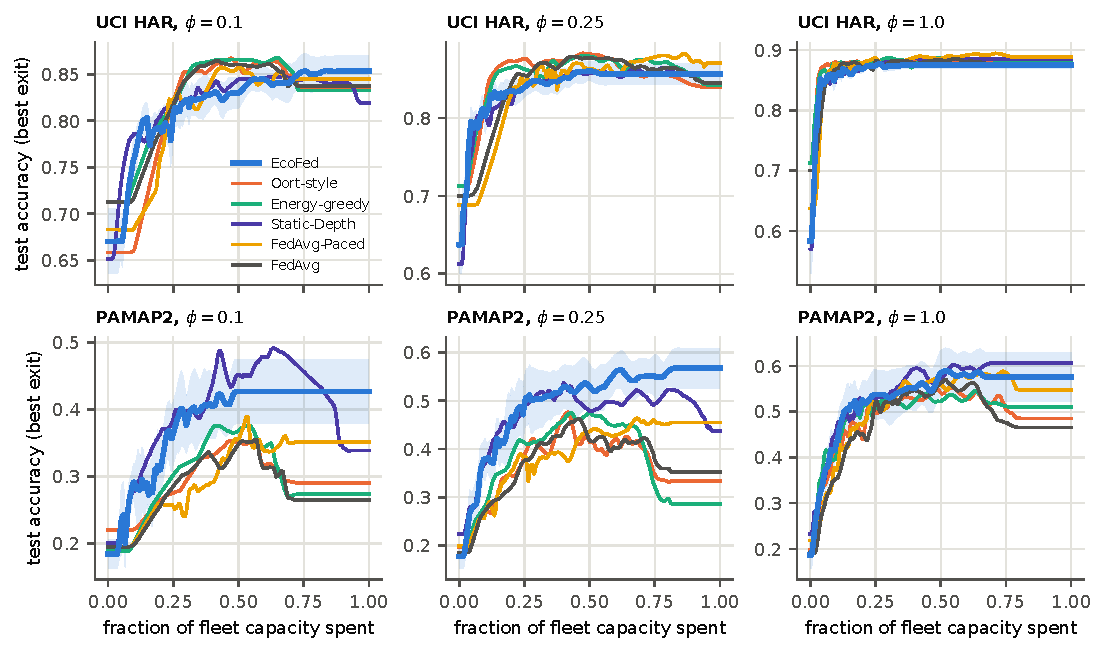
\includegraphics[width=\textwidth]{fig4_accuracy_vs_energy}
\caption{Test accuracy (best exit) against the fraction of fleet capacity spent; mean over seeds, shaded band is the 95\% CI of EcoFed. Methods that stop early keep their final accuracy; energy-blind baselines peak and then lose accuracy when batteries run out and the surviving clients dominate the aggregate.}\label{fig:curves}
\end{figure}

\paragraph{Strongly non-IID data and a binding budget (PAMAP2, $\phi\le0.25$): large gains}
At $\phi=0.25$ the final accuracy of EcoFed is 55.9\%, against 28.7--45.5\% for the baselines. The paired differences are $+10.4$ to $+27.2$ pp and significant against all seven baselines, including Static-Depth ($+12.1$ pp, 95\% CI $[8.3,15.9]$). With early stopping the margin shrinks but remains significant against six of seven baselines ($+7.3$ to $+10.9$ pp); Static-Depth is within noise ($+2.0$ pp, CI $[-2.3,6.6]$). At $\phi=0.1$ the final accuracy is again significantly higher than for every baseline ($+5.9$ to $+15.3$ pp), but the picture with early stopping reverses against the one baseline that never trains deep blocks: Static-Depth reaches 48.7\% at its best checkpoint against 41.0\% for EcoFed ($-7.8$ pp, CI $[-12.8,-3.0]$, Holm $p=0.068$). That baseline's final accuracy is 33.9\%: after its peak the accuracy of every energy-blind method falls while the fleet's batteries run out (Fig.~\ref{fig:curves}, bottom left), which is consistent with the surviving clients dominating a strongly label-skewed aggregate, although we did not isolate this cause. Its last exit is also essentially untrained (9.1\% accuracy at exit 4 against 37.5\% for EcoFed). Static-Depth is therefore a strong competitor at the tightest budget if the operator can detect the peak and stop; EcoFed is the better choice if the deployed model must also have usable deep exits, or if training cannot be stopped at the best checkpoint.

\paragraph{Loose budget (PAMAP2, $\phi=1$): parity with the best heuristics, less energy}
With energy no longer scarce the best-checkpoint accuracies of EcoFed (57.8\%), Static-Depth (58.7\%), single-exit FedAvg (58.4\%) and FedAvg-Paced (58.1\%) are indistinguishable (EcoFed is within $0.9$ pp of Static-Depth and $0.3$ pp of FedAvg-Paced, Holm $p=1.0$ for both), while EcoFed's final accuracy is significantly higher than that of FedAvg, FedProx, FedAvg-Q8, Oort-style and Energy-greedy ($+5.7$ to $+11.9$ pp). EcoFed spends 473~J against 511--570~J for the baselines other than Static-Depth (470~J).

\paragraph{Near-IID labels (UCI HAR): equal accuracy at much lower energy, but a small accuracy cost}
In UCI HAR all clients see all six activities, only the sensor placement and the person change, and every method reaches 84--89\% accuracy after a few rounds (Fig.~\ref{fig:curves}, top). EcoFed's final accuracy is statistically indistinguishable from the baselines at $\phi=0.1$ and $0.25$ and 1.8 pp below FedAvg-Paced at $\phi=1$ (significant). At the validation-selected checkpoint it is up to 2.7 pp lower than the multi-exit baselines (significant against FedAvg, FedProx and FedAvg-Paced at $\phi=0.25$ only) and 2.3--3.4 pp lower than single-exit FedAvg. In exchange it spends 1.6 times (at $\phi=0.25$) and 2.2 times (at $\phi=1$) less fleet energy than FedAvg over the run, and only 0.8--2.3\% of devices end below 2\% of battery capacity against 17--31\% for the energy-blind methods. At $\phi=0.1$ the picture is different: the baselines stop early because the remaining batteries cannot afford a full-depth round (they leave 28\% of the capacity stranded), whereas EcoFed uses 86\% of the capacity and ends with 19.5\% of the devices drained; this is the price of using the energy that is there.

\subsection{Energy to reach a target accuracy}
Fig.~\ref{fig:eta} reports the fleet energy needed to reach 90\% of the accuracy that FedAvg reaches when energy is not scarce. On UCI HAR, EcoFed reaches the target with 8.0~J at $\phi=0.1$ and $0.25$ and 16.5~J at $\phi=1$, which is 1.4 to 3.8 times less than FedAvg, FedProx, FedAvg-Q8 and FedAvg-Paced (significant in 11 of 12 comparisons; the exception is FedAvg-Paced at $\phi=0.1$, ratio 1.43, Holm $p=0.064$), and 1.6 to 2.2 times less than Oort-style and Energy-greedy at $\phi\le0.25$. At $\phi=1$ Oort-style and Energy-greedy are faster by about 20\% (12.9~J against 16.5~J; not significant after correction). Static-Depth is statistically tied with EcoFed on this metric on both datasets. On PAMAP2 the target is not always reached within the horizon (at $\phi=0.1$ 4 of 16 seeds for FedAvg and 9 of 16 for EcoFed, against 14 of 16 for Static-Depth), so the ratios are computed on the seeds in which both methods reach it: at $\phi=0.25$ EcoFed needs 1.9--2.5 times less energy than every baseline except Static-Depth (ratio 1.02).

\begin{figure}[t]
\centering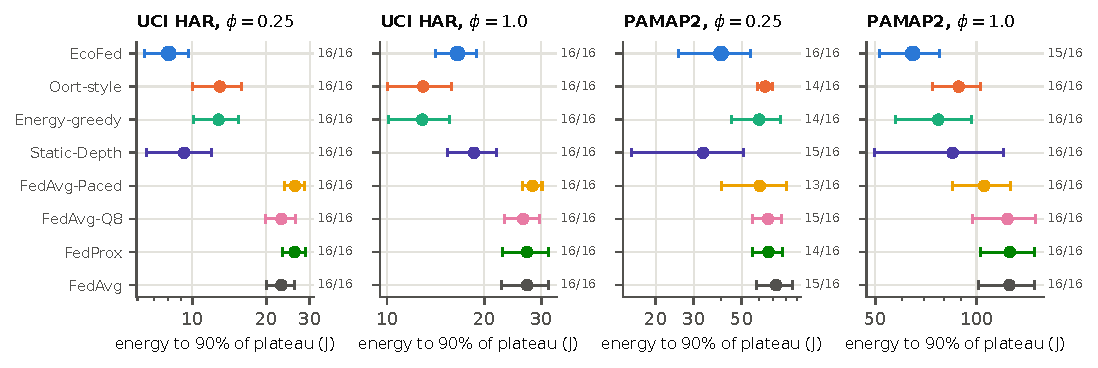
\includegraphics[width=\textwidth]{fig5_eta}
\caption{Fleet energy to reach 90\% of the FedAvg plateau (mean with 95\% CI over the seeds that reach it; the fraction on the right is the number of seeds that reach it).}\label{fig:eta}
\end{figure}

\subsection{Where the gains come from: ablations}\label{sec:ablation}
Table~\ref{tab:ablation} removes one ingredient at a time (8 seeds). Differences are paired by seed; $p$-values below are unadjusted paired $t$-tests and should be read as descriptive.

\begin{table}[t]
\centering\scriptsize
\caption{Ablations of EcoFed (mean $\pm$ 95\% CI over 8 seeds). Exit-4 acc.: test accuracy of the last exit, which is only trained by clients that reach full depth.}\label{tab:ablation}
\setlength{\tabcolsep}{3pt}
\resizebox{\textwidth}{!}{\begin{tabular}{@{}llrrrrr@{}}
\toprule
Data / $\phi$ & Variant & Acc@25\% & Acc@100\% & AUC & Exit-4 acc. & mean depth\\
\midrule
UCI HAR, 0.1 & EcoFed & 83.4\,$\pm$\,1.3 & 87.1\,$\pm$\,0.9 & 83.1\,$\pm$\,0.7 & 86.4\,$\pm$\,0.9 & 1.80\\
 & EcoFed w/o energy queue & 55.2\,$\pm$\,2.7 & 79.5\,$\pm$\,3.3 & 70.0\,$\pm$\,1.8 & 79.6\,$\pm$\,3.8 & 1.59\\
 & EcoFed w/o coverage queue & 84.6\,$\pm$\,1.5 & 85.0\,$\pm$\,2.3 & 82.8\,$\pm$\,1.8 & 76.4\,$\pm$\,14.6 & 1.17\\
 & EcoFed, fixed depth & 76.2\,$\pm$\,4.9 & 77.7\,$\pm$\,3.5 & 73.7\,$\pm$\,3.3 & 78.4\,$\pm$\,3.0 & 1.01\\
 & EcoFed, fixed precision & 83.5\,$\pm$\,2.3 & 86.8\,$\pm$\,1.5 & 83.2\,$\pm$\,1.3 & 86.3\,$\pm$\,1.7 & 1.59\\
 & EcoFed, fixed epochs & 83.9\,$\pm$\,1.8 & 86.2\,$\pm$\,1.9 & 82.2\,$\pm$\,1.2 & 85.2\,$\pm$\,2.3 & 1.49\\
\midrule
UCI HAR, 0.25 & EcoFed & 85.2\,$\pm$\,1.1 & 87.4\,$\pm$\,1.2 & 85.6\,$\pm$\,1.1 & 87.7\,$\pm$\,1.0 & 2.56\\
 & EcoFed w/o energy queue & 67.4\,$\pm$\,4.6 & 80.8\,$\pm$\,3.7 & 78.7\,$\pm$\,1.7 & 81.2\,$\pm$\,3.2 & 2.66\\
 & EcoFed w/o coverage queue & 84.8\,$\pm$\,2.4 & 87.2\,$\pm$\,2.0 & 86.3\,$\pm$\,1.8 & 58.8\,$\pm$\,27.1 & 1.23\\
 & EcoFed, fixed depth & 69.3\,$\pm$\,4.1 & 69.3\,$\pm$\,4.1 & 68.9\,$\pm$\,4.0 & 61.6\,$\pm$\,7.1 & 0.53\\
 & EcoFed, fixed precision & 86.0\,$\pm$\,1.6 & 88.3\,$\pm$\,1.3 & 85.6\,$\pm$\,1.2 & 88.5\,$\pm$\,1.4 & 2.37\\
 & EcoFed, fixed epochs & 84.9\,$\pm$\,1.3 & 88.1\,$\pm$\,1.5 & 85.4\,$\pm$\,1.3 & 88.1\,$\pm$\,1.7 & 2.33\\
\midrule
PAMAP2, 0.1 & EcoFed & 36.7\,$\pm$\,4.1 & 42.0\,$\pm$\,4.5 & 38.5\,$\pm$\,3.4 & 35.4\,$\pm$\,5.3 & 1.76\\
 & EcoFed w/o energy queue & 25.9\,$\pm$\,2.5 & 32.4\,$\pm$\,13.3 & 33.6\,$\pm$\,3.3 & 21.8\,$\pm$\,7.5 & 1.40\\
 & EcoFed w/o coverage queue & 28.2\,$\pm$\,6.9 & 27.5\,$\pm$\,6.2 & 27.2\,$\pm$\,5.9 & 14.0\,$\pm$\,4.6 & 0.80\\
 & EcoFed, fixed depth & 26.9\,$\pm$\,4.2 & 26.9\,$\pm$\,4.2 & 26.4\,$\pm$\,4.1 & 23.9\,$\pm$\,4.3 & 0.55\\
 & EcoFed, fixed precision & 32.6\,$\pm$\,5.5 & 38.9\,$\pm$\,8.6 & 35.1\,$\pm$\,7.2 & 35.3\,$\pm$\,7.3 & 1.66\\
 & EcoFed, fixed epochs & 33.1\,$\pm$\,6.3 & 33.8\,$\pm$\,4.9 & 30.3\,$\pm$\,5.0 & 27.0\,$\pm$\,8.5 & 1.17\\
\midrule
PAMAP2, 0.25 & EcoFed & 50.8\,$\pm$\,4.8 & 57.5\,$\pm$\,3.6 & 50.5\,$\pm$\,3.7 & 49.2\,$\pm$\,3.9 & 2.59\\
 & EcoFed w/o energy queue & 30.8\,$\pm$\,3.3 & 28.9\,$\pm$\,6.7 & 38.7\,$\pm$\,4.6 & 23.7\,$\pm$\,5.9 & 2.55\\
 & EcoFed w/o coverage queue & 50.1\,$\pm$\,9.9 & 56.7\,$\pm$\,8.6 & 52.3\,$\pm$\,7.3 & 25.7\,$\pm$\,3.7 & 1.64\\
 & EcoFed, fixed depth & 35.8\,$\pm$\,4.1 & 40.9\,$\pm$\,9.8 & 37.4\,$\pm$\,7.2 & 32.7\,$\pm$\,8.7 & 2.36\\
 & EcoFed, fixed precision & 47.8\,$\pm$\,7.5 & 55.3\,$\pm$\,6.4 & 49.4\,$\pm$\,5.4 & 48.5\,$\pm$\,4.8 & 2.54\\
 & EcoFed, fixed epochs & 40.5\,$\pm$\,7.3 & 53.6\,$\pm$\,7.5 & 45.4\,$\pm$\,6.0 & 40.9\,$\pm$\,6.6 & 2.51\\
\midrule
Speech Commands, 0.1 & EcoFed & 31.0\,$\pm$\,1.2 & 36.1\,$\pm$\,1.2 & 33.4\,$\pm$\,0.8 & 31.9\,$\pm$\,3.4 & 1.04\\
 & EcoFed w/o energy queue & 28.7\,$\pm$\,2.4 & 33.0\,$\pm$\,0.8 & 30.6\,$\pm$\,0.8 & 30.7\,$\pm$\,2.9 & 0.78\\
 & EcoFed w/o coverage queue & 30.2\,$\pm$\,2.9 & 39.8\,$\pm$\,4.0 & 34.6\,$\pm$\,2.0 & 30.6\,$\pm$\,7.8 & 1.02\\
 & EcoFed, fixed depth & 29.7\,$\pm$\,2.4 & 30.7\,$\pm$\,3.5 & 30.1\,$\pm$\,1.9 & 29.9\,$\pm$\,4.2 & 0.83\\
 & EcoFed, fixed precision & 29.2\,$\pm$\,2.3 & 34.6\,$\pm$\,2.5 & 32.5\,$\pm$\,1.1 & 30.8\,$\pm$\,5.3 & 1.04\\
 & EcoFed, fixed epochs & 29.8\,$\pm$\,1.9 & 35.3\,$\pm$\,1.9 & 32.7\,$\pm$\,1.2 & 32.0\,$\pm$\,4.5 & 0.94\\
\midrule
Speech Commands, 0.25 & EcoFed & 37.5\,$\pm$\,1.3 & 42.8\,$\pm$\,1.3 & 40.2\,$\pm$\,1.1 & 41.0\,$\pm$\,2.2 & 1.54\\
 & EcoFed w/o energy queue & 29.9\,$\pm$\,2.1 & 34.6\,$\pm$\,1.1 & 32.0\,$\pm$\,0.9 & 33.2\,$\pm$\,3.1 & 1.75\\
 & EcoFed w/o coverage queue & 39.8\,$\pm$\,1.9 & 42.4\,$\pm$\,3.0 & 40.4\,$\pm$\,2.4 & 10.4\,$\pm$\,8.2 & 1.01\\
 & EcoFed, fixed depth & 26.4\,$\pm$\,6.4 & 26.4\,$\pm$\,6.4 & 26.4\,$\pm$\,6.4 & 21.7\,$\pm$\,10.1 & 0.21\\
 & EcoFed, fixed precision & 37.3\,$\pm$\,1.2 & 41.0\,$\pm$\,1.8 & 38.5\,$\pm$\,1.6 & 36.7\,$\pm$\,3.6 & 1.26\\
 & EcoFed, fixed epochs & 39.4\,$\pm$\,1.8 & 41.1\,$\pm$\,1.6 & 39.6\,$\pm$\,1.6 & 40.2\,$\pm$\,2.5 & 1.26\\
\bottomrule
\end{tabular}}
\end{table}

\emph{The energy queue is essential.} Without it clients keep running expensive configurations until their batteries are empty: 42--82 pp more devices end drained, 29--56 J more energy is spent at $\phi=0.25$, and final accuracy drops by 4.7--24.6 pp (all four settings, $p\le0.006$). \emph{Depth and epoch control matter more than precision control.} Forcing full depth lowers final accuracy by 3.3 to 18.6 pp (significant in three of the four settings; 26 to 83 J less energy is used because clients cannot afford it); forcing two epochs costs 1.6 to 10.6 pp (significant only at HAR $\phi=0.25$). Forcing 32-bit uploads changes accuracy by at most 1.9 pp and is never significant; this is expected given the energy breakdown of Fig.~\ref{fig:energy}, where radio energy is a small share of the cost of a participation in our default setting. We return to this in Section~\ref{sec:sens}. \emph{The coverage queue protects the deep exits.} Without it the last exit loses 21.0 pp on PAMAP2 at $\phi=0.1$ ($p<0.001$; final accuracy $-12.1$ pp, $p=0.012$), 6.0 pp at $\phi=0.25$ and 4.2 pp on HAR at $\phi=0.1$ ($p=0.03$); at looser budgets the effect is within noise. The best-checkpoint accuracy does not suffer (shallow exits are enough to classify), so the coverage queue matters for the quality of the whole multi-exit model rather than for the accuracy of its best exit. This is the behaviour the theory predicts and we test it directly next.

\begin{figure}[t]
\centering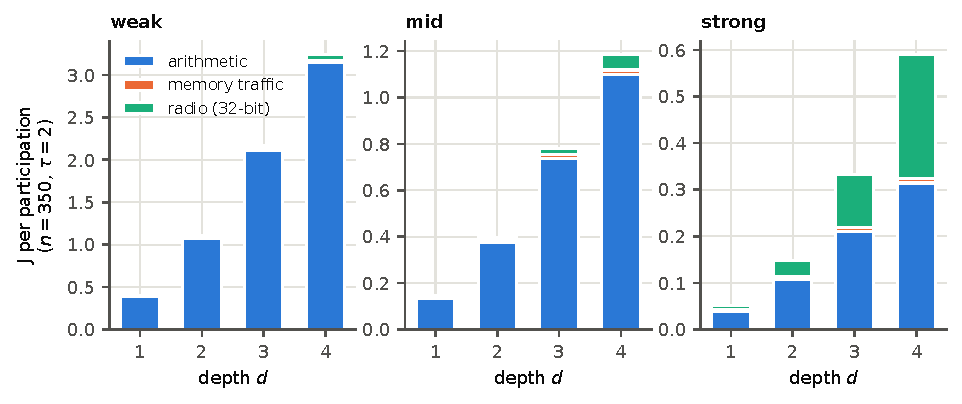
\includegraphics[width=0.9\textwidth]{fig3_energy_decomposition}
\caption{Modelled energy of one participation ($n=350$ samples, 2 epochs, 32-bit upload) by depth, split into arithmetic, memory traffic and radio, for the three device classes. For this small network on-device arithmetic dominates; radio energy is visible only for the LTE-class device.}\label{fig:energy}
\end{figure}

\subsection{The coverage floor is visible in the data}\label{sec:coverage-exp}
Theorem~\ref{thm:main} predicts that, for a fixed horizon, the final gradient norm grows with $(1-\sigma)^2$. We test this with a controlled probe that removes every other source of variation: no energy limit, uniform client sampling, and a depth that is $L=4$ with probability $\sigma$ and $1$ otherwise, so that $\Pr[d\ge j]=\sigma$ for $j\ge2$ (6 seeds $\times$ 8 values of $\sigma$ $\times$ 2 datasets, 100 rounds). Fig.~\ref{fig:cov} shows the squared norm of the gradient of the full multi-exit objective at the final iterate. It rises with $(1-\sigma)^2$ on both datasets: the linear fit has slope $0.88$ and $R^2=0.14$ on UCI HAR (Spearman $\rho=0.30$, $p=0.037$) and slope $18.7$ and $R^2=0.24$ on PAMAP2 ($\rho=0.51$, $p=2\times10^{-4}$). The relation is noisy and the bound is not tight---we do not claim it is---but the sign, the monotone trend and the quadratic shape are what the theorem predicts, and the last-exit accuracy falls accordingly (from 90.3\% at $\sigma=1$ to 87.6\% at $\sigma=0.1$ on UCI HAR; Fig.~\ref{fig:cov}, right). Note that the practical aggregator used in the experiments is the sample-normalised average, not the Horvitz--Thompson weighting of the analysis; the probe therefore tests the prediction for the aggregator that is actually deployed.

\begin{figure}[t]
\centering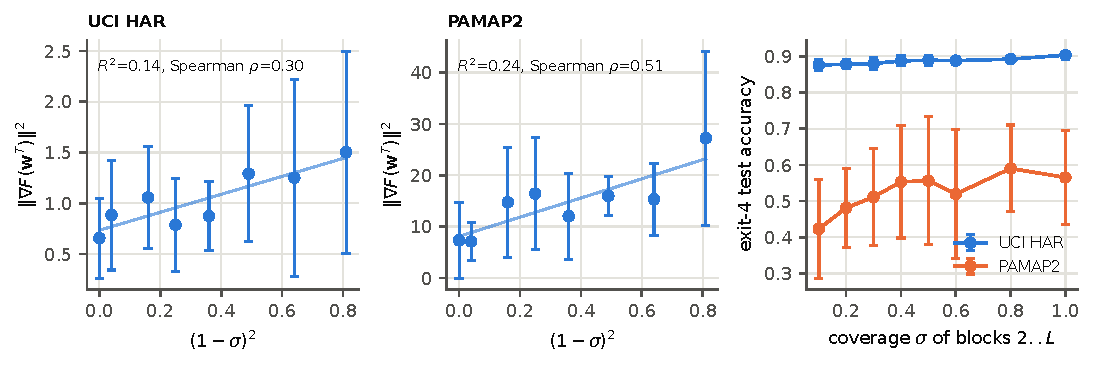
\includegraphics[width=\textwidth]{fig6_coverage_floor}
\caption{Coverage probe. Left and middle: squared full-objective gradient norm at the final iterate against $(1-\sigma)^2$ (mean and 95\% CI over 6 seeds, with a least-squares line over the individual runs). Right: last-exit test accuracy against the coverage $\sigma$ of the deep blocks.}\label{fig:cov}
\end{figure}

\subsection{An energy--accuracy frontier from one knob}\label{sec:pareto}
The shadow price $\lambda$ of Eq.~\eqref{eq:score} moves EcoFed along an energy--accuracy frontier, whereas a baseline's operating point is simply the one at which it stops. Fig.~\ref{fig:pareto} shows the validation-selected checkpoint (accuracy against the fleet energy spent up to it) for four values of $\lambda$ with all other settings fixed at their tuned values, on the first eight evaluation seeds; the sweep is reported in full and was not used to select anything, and the baselines in the figure are the same eight seeds.

\textbf{UCI HAR.} At $\phi=1$, $\lambda=0.3$ (the tuned value) reaches 88.4\% with 100~J, within 0.3 pp of FedAvg-Q8 (88.6\%, 138~J) and FedAvg-Paced (88.7\%, 171~J) and equal to FedAvg (88.3\%, 228~J), i.e.\ 27\% to 56\% less energy for essentially the same accuracy; $\lambda=1$ gives 86.1\% with 74~J. At $\phi=0.25$ the curve is on top of the baselines: $\lambda=0.03$ reaches 88.1\% with 86~J, against 87.5\% with 67~J for FedAvg and 87.8\% with 87~J for FedAvg-Q8.
\textbf{PAMAP2.} At $\phi=0.25$ the tuned setting ($\lambda=0.1$) reaches 57.8\% with 141~J and lies above every baseline (best baseline: Static-Depth 54.7\% with 108~J; best energy-blind baseline 48.1\%). At $\phi=1$ it does not: $\lambda=0.03$ gives 56.3\% with 446~J and the tuned $\lambda=0.1$ gives 54.1\% with 331~J, below Static-Depth (58.4\%, 348~J) and FedAvg-Q8 (60.4\%, 417~J).
\textbf{Speech Commands.} At $\phi=0.25$ the best EcoFed point is 48.8\% with 19~J ($\lambda=0.1$), against 53.2\% with 19~J for FedAvg-Paced and 47.5\% with 19--23~J for FedAvg-Q8 and Static-Depth; at $\phi=1$ the lowest price gives 59.5\% with 84~J, 0.4 to 5 pp below the baselines (59.9--64.5\% with 86--93~J).

In short, the frontier lies on or above the baselines on UCI HAR and on PAMAP2 at the binding budget, where it saves energy or accuracy, and below the best baselines at the loose budget on PAMAP2 and on Speech Commands. The lower accuracy of the tuned EcoFed at $\phi=1$ in Table~\ref{tab:main} is partly a matter of operating point: the price selected at $\phi=0.25$ is too frugal for $\phi=1$ (the sweep shows a higher accuracy at $\lambda=0.03$ for PAMAP2 and Speech Commands). Retuning $\phi=1$ separately is the obvious fix and would be fairer to EcoFed; we did not do it because of its computational cost.

\begin{figure}[t]
\centering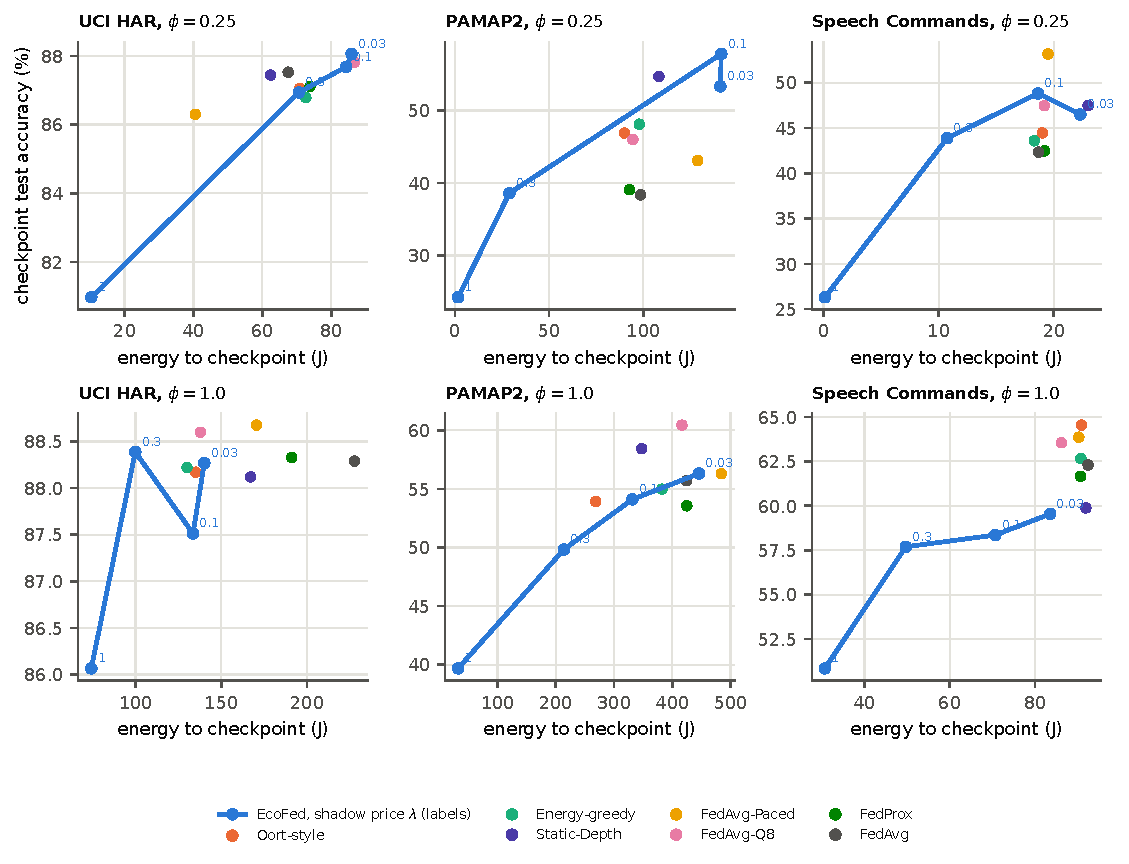
\includegraphics[width=\textwidth]{fig10_pareto}
\caption{Energy--accuracy frontier at the validation-selected checkpoint. Line: EcoFed with shadow price $\lambda\in\{0.03,0.1,0.3,1\}$ (labels); dots: baselines at their tuned settings. All points are means over the first eight seeds.}\label{fig:pareto}
\end{figure}


\subsection{Robustness to the energy model}\label{sec:sens}
Because energy is modelled, we ask how much the conclusions depend on the model (Fig.~\ref{fig:sens}; PAMAP2, $\phi=0.25$, 8 seeds, metric: area under test accuracy as a function of the energy fraction spent).

\paragraph{Radio-to-compute cost ratio}
Multiplying all radio energies by 10 or 100 turns communication from a minor into a major cost. EcoFed's area under the curve falls from 48.7\% to 45.3\% and 43.0\% (a loss of 5.7 pp), while FedAvg, FedAvg-Q8, Oort-style and Energy-greedy fall from 35.0--36.1\% to 20.9--23.7\% (losses of 12.4 to 14.1 pp). Even FedAvg-Q8, which quantises uploads to 8 bits, loses 12.6 pp, because it still sends the entire network; EcoFed can reduce the bits sent by choosing a smaller depth as well as a smaller bit-width. So precision control, which is irrelevant in the default setting (Section~\ref{sec:ablation}), becomes useful together with depth control when radio energy dominates.

\paragraph{Wrong energy beliefs}
We let the energy that actually drains the batteries differ from the controller's belief by independent log-normal factors on the arithmetic and memory constants of every device ($\sigma=0.25$ and $0.5$). EcoFed's area under the curve is 48.7\%, 50.2\% and 48.7\% for $\sigma=0,0.25,0.5$---unchanged within the seed-to-seed variation---which is what one expects when queues integrate the energy that devices report rather than the energy that the model predicts. The other methods are also fairly insensitive (changes of at most 2.4 pp, for Oort-style; Static-Depth does not change). The batteries, not the controllers' beliefs, are the binding constraint for the baselines, and they are battery-aware by construction, so this experiment shows that EcoFed is not \emph{more} fragile than they are rather than that it is more robust.

\paragraph{Unmodelled per-sample overhead}
Section~\ref{sec:latency} shows that on a real CPU a participation costs a fixed amount per sample on top of the MAC-proportional part, equivalent to 0.55--0.75 million MACs. We add 0.5 and 1.0 million MAC-equivalents per training sample to the \emph{true} energy only. On PAMAP2 EcoFed's area under the curve falls from 48.7\% to 45.1\% and 42.6\%, Static-Depth's from 43.7\% to 41.6\% and 40.0\%, and FedAvg-Paced's from 37.5\% to 36.2\% and 36.4\%. EcoFed loses more than the others (6.1 pp against 3.7 and 1.1 pp) because it relies on shallow updates being cheap, but it stays ahead (by 3.5 and 2.6 pp over Static-Depth and by 8.9 and 6.2 pp over FedAvg-Paced). On UCI HAR, where all methods are within about 3 pp, EcoFed's area (83.1\%, 82.5\%) is 0.6 and 2.7 pp below FedAvg-Paced's (83.7\%, 85.2\%) and above Static-Depth's (81.4\%, 80.5\%). A cost model that overstates the benefit of shallow updates therefore reduces, but does not remove, the advantage of depth control, and the closed-loop queues keep the batteries safe.

\begin{figure}[t]
\centering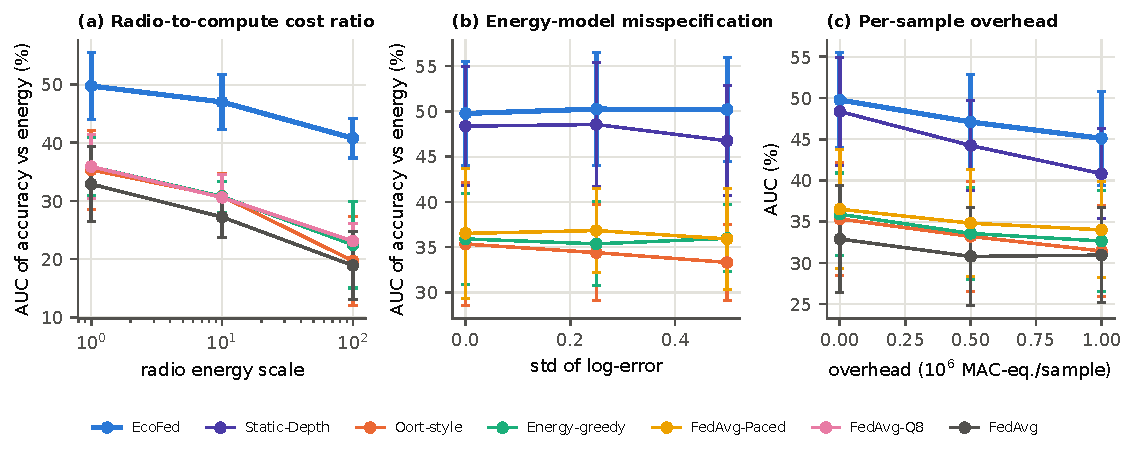
\includegraphics[width=\textwidth]{fig7_sensitivity}
\caption{Sensitivity of the area under the accuracy-versus-energy curve on PAMAP2 at $\phi=0.25$ (mean and 95\% CI over 8 seeds). (a) Radio energy scaled by 1, 10, 100. (b) Log-normal error between the energy constants assumed by the controller and the true ones. (c) Unmodelled per-sample overhead added to the true energy.}\label{fig:sens}
\end{figure}


\subsection{Lifecycle energy}\label{sec:lifecycle}
Training is only half of the energy bill. We deploy each trained model with the confidence-gated cascade of Section~\ref{sec:lifecycle-model}: a single threshold $\theta$ per model is chosen on validation data as the cheapest one whose validation accuracy is within one percentage point of the model's best single exit, and we then report test accuracy and modelled inference energy (fleet-average device mix). Table~\ref{tab:life} compares three deployments: single-exit FedAvg (trained with a last-exit loss; every window runs the full network), multi-exit FedAvg with the cascade, and EcoFed with the cascade. For a fleet that classifies one 2.56~s window every 1.28~s per device, always on, the last column gives the time after which the energy spent on serving exceeds the energy spent on training ($M_\times$ divided by the fleet's window rate).

\begin{table}[t]
\centering\scriptsize
\caption{Lifecycle energy (means over 16 seeds). Test acc.: accuracy of the deployed cascade (single exit for the first row). $E_{train}$: fleet energy used for training. $\bar e_{inf}$: expected inference energy per window. $M_\times=E_{train}/\bar e_{inf}$: number of inferences after which serving costs as much as training did.}\label{tab:life}
\setlength{\tabcolsep}{3pt}
\resizebox{\textwidth}{!}{\begin{tabular}{@{}llrrrrrr@{}}
\toprule
Data / $\phi$ & Model & Test acc. (\%) & $E_{train}$ (J) & $\bar e_{inf}$ ($\mu$J) & exits at 1 (\%) & $M_\times$ ($10^5$) & days to $M_\times$\\
\midrule
UCI HAR, 0.25 & FedAvg, single exit & 87.2 & 116.1 & 845 & 0 & 1.37 & 0.13\\
 & FedAvg, cascade & 83.9 & 116.1 & 250 & 31 & 4.65 & 0.43\\
 & EcoFed, cascade & 85.6 & 70.7 & 114 & 98 & 6.19 & 0.57\\
\midrule
UCI HAR, 1.0 & FedAvg, single exit & 89.1 & 378.9 & 845 & 0 & 4.49 & 0.42\\
 & FedAvg, cascade & 86.5 & 378.9 & 209 & 48 & 18.16 & 1.68\\
 & EcoFed, cascade & 86.4 & 176.5 & 169 & 86 & 10.47 & 0.97\\
\midrule
PAMAP2, 0.25 & FedAvg, single exit & 31.4 & 136.2 & 950 & 0 & 1.43 & 0.11\\
 & FedAvg, cascade & 32.7 & 136.2 & 611 & 7 & 2.23 & 0.17\\
 & EcoFed, cascade & 54.5 & 148.2 & 378 & 73 & 3.92 & 0.29\\
\midrule
PAMAP2, 1.0 & FedAvg, single exit & 47.6 & 555.9 & 950 & 0 & 5.85 & 0.43\\
 & FedAvg, cascade & 46.6 & 555.9 & 450 & 22 & 12.36 & 0.92\\
 & EcoFed, cascade & 58.6 & 472.8 & 436 & 55 & 10.85 & 0.80\\
\bottomrule
\end{tabular}}
\end{table}

Three observations follow. First, \emph{inference energy per window can be cut by a factor of 2 to 7 by the cascade.} EcoFed's cascade needs 114 and 169~$\mu$J per window on UCI HAR against 845~$\mu$J for the single-exit network (7.4 and 5.0 times less), at a cost of 1.6 and 2.7 pp of accuracy at $\phi=0.25$ and $1$; on PAMAP2 it needs 378 and 436~$\mu$J against 950~$\mu$J (2.5 and 2.2 times less) with a \emph{higher} accuracy (54.5\% and 58.6\% against 31.4\% and 47.6\% for single-exit FedAvg, the latter being poorly trained under the same budget). The multi-exit FedAvg cascade saves less (1.6 to 4.0 times) because its shallow exits are weaker: only 7--48\% of windows leave at the first exit, against 55--98\% for EcoFed. Table~\ref{tab:exits} shows why: with exit weights $\lambda_j\propto j^2$ the first exit receives only 3.3\% of the loss weight of a full-depth client, and FedAvg's first exit reaches 55.9\% on UCI HAR against 85.3\% for EcoFed, whose depth-1 clients train it with the full loss weight. This is a consequence of our choice of exit weights (made to favour the last exit, \ref{app:extra}); with uniform weights the shallow exits of the energy-blind baselines would be better and their last exit worse, so the cascade comparison should be read with that choice in mind. Second, \emph{the extra training cost of a multi-exit model is negligible.} At $\phi=0.25$ on PAMAP2 EcoFed trains with 12~J more than FedAvg (148 against 136~J) but saves 572~$\mu$J per window relative to single-exit FedAvg; by Eq.~\eqref{eq:breakeven} the extra training energy is repaid after about $2.1\times10^4$ windows, i.e.\ about 22 minutes of operation of the 20-device fleet. On UCI HAR and at $\phi=1$ EcoFed trains with \emph{less} energy than FedAvg and also serves with less, so $M^\star\le0$. Third, \emph{serving dominates the lifecycle.} In every row serving matches the training energy within $0.1$ to $1.7$ days of fleet operation (Table~\ref{tab:life}, last column; Fig.~\ref{fig:life}), and over a month of operation inference would use roughly 18 to 270 times the energy of training. Savings in the training phase are therefore worth having mainly because they come with models whose deployed cost is also lower; the largest lever on the total energy is the exit policy.

\begin{figure}[t]
\centering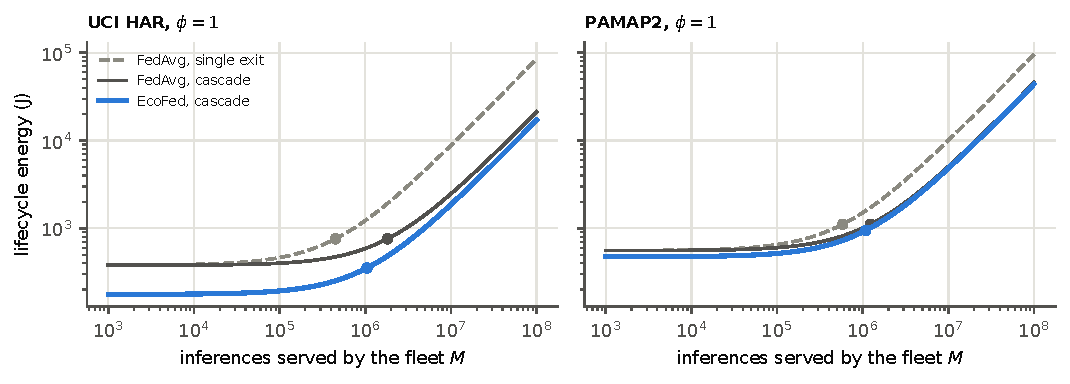
\includegraphics[width=\textwidth]{fig9_lifecycle}
\caption{Lifecycle energy against the number of inferences served by the fleet ($\phi=1$). Dots mark $M_\times$, where inference energy equals training energy.}\label{fig:life}
\end{figure}


\subsection{Controller overhead}\label{sec:overhead}
\paragraph{Controller cost}
EcoFed scores $|\mathcal C|=16$ configurations per client and sorts the best scores. Fig.~\ref{fig:scaling}a reports the measured time of the selection step in our (unoptimised, pure Python) implementation on synthetic fleets with 5\% of clients selected: 3~ms for $N=100$, 0.036~s for $N=10^3$, 0.26~s for $N=10^4$ and 2.7~s for $N=10^5$, 2.6 times the cost of an Oort-style top-$m$ ranking at $N=10^5$ (1.0~s) and 8 to 14 times at $N\le10^4$. This is negligible compared with a federated round, which takes seconds to minutes at that scale, but it is a Python measurement of the selection step only and says nothing about the scalability of learning itself, which we did not test beyond 20 clients.

\subsection{Cost model versus measured latency}\label{sec:latency}
The relative cost of depth is the lever behind depth control, so we checked it against wall-clock time. We timed one training step of the multi-exit network at depths 1--4 on a single CPU thread (batch 32, median of 40 repetitions). Measured time per sample grows more slowly than the modelled cost: depth 4 takes 3.4 times as long as depth 1 on UCI HAR's 9-channel input and 3.1 times on PAMAP2's 18-channel input, while the MAC count grows by a factor of 8.1 and 4.6 (Fig.~\ref{fig:scaling}b). A linear model of time in MACs fits well ($R^2=0.96$ and $0.98$) with a fixed cost per sample equivalent to about 0.75 and 0.55 million MACs. We therefore do not claim that the modelled savings from shallow updates are what a CPU would show; the sensitivity experiment of Section~\ref{sec:sens} injects that overhead into the true energy and shows that EcoFed's advantage on PAMAP2 shrinks but persists. Latency is not energy, and an accelerator would behave differently; this check only validates the \emph{relative} depth scaling on one CPU.

\begin{figure}[t]
\centering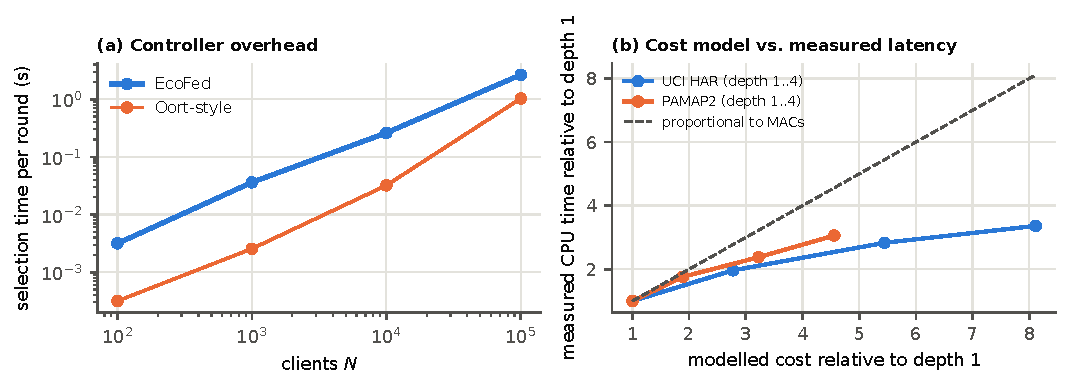
\includegraphics[width=\textwidth]{fig11_system}
\caption{(a) Time of the selection step against the number of clients (5\% selected; synthetic fleets; one CPU core). (b) Measured CPU time per training sample against the modelled cost, both relative to depth 1; the dashed line is proportionality.}\label{fig:scaling}
\end{figure}


\section{Discussion}\label{sec:discussion}

\paragraph{What the evidence supports}
Three findings are supported by paired statistics over 16 seeds. First, when the budget is binding and the data are strongly label-skewed across clients (PAMAP2, $\phi\le0.25$), letting clients choose how much of the network to train, under energy prices and a coverage constraint, gives a much better final model than FedAvg-type training with random or utility-based selection (+6 to +27 pp). Second, when the labels are similar across clients (UCI HAR) the same control gives the same accuracy within 1--3 pp for $1.6$--$2.2$ times less energy and with far fewer drained devices. Third, the pieces that matter are the energy queue, depth control and epoch control; the coverage queue matters for the deep exits, and precision control matters little unless radio energy is expensive relative to computation (Section~\ref{sec:sens}). The theory is consistent with the coverage experiment, although the relation is noisy and the bound is loose.

\paragraph{What it does not support}
EcoFed does not dominate. Static-Depth---a one-line rule that gives each device the deepest depth that fits its budget---reaches the best checkpoint accuracy on PAMAP2 at the tightest budget ($+7.8$ pp over EcoFed) and ties EcoFed at the loosest, and its energy to a target accuracy is statistically indistinguishable from EcoFed's. What EcoFed adds over that rule is accuracy at the \emph{end} of the run, usable deep exits, protection of the batteries and a single knob, $\lambda$, that trades energy for accuracy (Section~\ref{sec:pareto}). On UCI HAR the most accurate method is single-exit FedAvg, which beats EcoFed by 2--3 pp at the best checkpoint; a multi-exit model is only worth its (small) extra training cost if the deployment-time savings of Section~\ref{sec:lifecycle} are wanted.

\paragraph{Why depth control may help when labels are skewed}
A plausible explanation, which we did not test in isolation, is breadth of participation: cheap shallow updates let many clients---and therefore many activities---contribute in every phase of the run, while full-depth updates exhaust a few clients and then let the fleet shrink to those that can afford them. The accuracy collapse of the energy-blind baselines after their peak on PAMAP2 and the near-parity on UCI HAR, where every client holds every label, are both consistent with this reading.

\paragraph{Implications for sustainable edge AI}
The lifecycle analysis reframes where the energy goes. In our model, a fleet that serves a wearable classifier continuously spends as much energy on inference as it spent on training within one to two days, and for the cascades and the PAMAP2 and UCI HAR models studied here 18 to 270 times as much over a month (Table~\ref{tab:life}). Two consequences follow. A federated training controller should be judged not only by the Joules it saves during training---which in absolute terms are small---but by whether it produces models that can be served cheaply: EcoFed's shallow exits are confident enough that 55--98\% of windows leave at the first block, while the exits of the model trained with a plain multi-exit FedAvg are not. And the training cost of making a model multi-exit is repaid within minutes of operation, so there is no energy argument for deploying the single-exit network, even where single-exit training reaches a slightly higher accuracy.


\paragraph{Practical guidance}
(i) Estimate the budget regime first: if the energy per participation of the full model is within a factor of a few of the per-round budget, depth and epoch control pay off; if energy is abundant, they only save energy. (ii) If the data are close to IID across clients, expect little accuracy to be lost by shallow, cheap updates, and use the savings. (iii) If the operator can stop training at a validation-selected checkpoint and does not need deep exits, a static capability-based depth is a strong, simple baseline. (iv) Keep the energy accounting closed-loop: EcoFed's queues use energy reported by the devices, which is what makes it robust to an incorrect energy model.

\section{Limitations and threats to validity}\label{sec:limits}
\begin{itemize}[leftmargin=1.4em,itemsep=1pt]
\item \textbf{Energy is modelled, not measured.} The device constants are assumptions and the paper contains no power measurement. Section~\ref{sec:sens} shows that conclusions are robust to radio cost, to multiplicative errors of up to 50\% (log-normal $\sigma=0.5$) in the controller's belief, and to an unmodelled per-sample overhead fitted from CPU latency; but a power-metered Raspberry Pi/Jetson study is the necessary next step (the measurement and fitting harness is provided, \ref{app:hardware}, but was not run), and the absolute Joules reported here should not be quoted as measurements.
\item \textbf{Scale.} The fleets have 16--20 clients and the network 27\,784 parameters; the selection is 5 clients per round over 80 rounds. We do not know how the ranking of methods changes with thousands of clients, deeper networks, or larger models; the controller overhead measurements (Section~\ref{sec:overhead}) say only that the algorithm itself scales.
\item \textbf{Two datasets from one domain.} Both are wearable inertial benchmarks. Results on audio or vision, and on datasets with feature rather than label skew, may differ.
\item \textbf{Tuning asymmetry.} Every method was tuned on separate seeds and validation subjects with a two-stage search, but EcoFed has more knobs (14 trials) than most baselines (3--7). Several selected values lie on the edge of their grid (for example the learning rate, and the depth exponent $\kappa_d=0.5$ for EcoFed), so all methods may be slightly under-tuned. The setting $\phi=1$ reuses the $\phi=0.25$ configuration. A pilot on tuning seeds showed that randomised instead of top-$m$ selection and $\kappa_d=0.25$ changed the validation AUC by between $-2.4$ and $+2.5$ points depending on the setting; we kept the pre-specified configuration rather than re-tune after seeing test results.
\item \textbf{Theory versus practice.} Theorem~\ref{thm:main} assumes iterate-independent participation, bounded gradients and an unbiased Horvitz--Thompson aggregator; the experiments use utility-based selection and sample-normalised block averages. Proposition~\ref{prop:lyap} is stated for an idealised system. The coverage experiment supports the qualitative prediction only.
\item \textbf{Exit weights.} We weight exits proportionally to $j^2$ for all methods. This favours the last exit and handicaps the shallow exits of full-depth methods, which affects the cascade comparison (Table~\ref{tab:exits}); we did not test other weightings beyond the pilot of \ref{app:extra}.
\item \textbf{Baselines.} Static-Depth and Oort-style are our simplified implementations of ideas from the literature, not reproductions of DepthFL/HeteroFL/ScaleFL or the Oort system.
\item \textbf{Validation-selected checkpoint.} The best-checkpoint metric assumes a small validation set at the server; the final-accuracy metric does not.
\item \textbf{Not modelled.} Stragglers and dropouts, wireless channel dynamics, charging, privacy mechanisms and security, and the energy of the server.
\end{itemize}

\section{Conclusion}\label{sec:conclusion}
We studied federated learning of multi-exit networks on battery-limited fleets, where energy is spent twice---when training and when serving. A convergence bound shows that letting weak devices train only shallow blocks creates an error floor controlled by how often each block is trained; EcoFed turns this into a coverage constraint and combines it with per-device energy queues and a shadow price in a controller that costs $O(N|\mathcal C|)$ per round. On two wearable benchmarks it improves the final accuracy of the federated model substantially when labels are strongly skewed and the budget binds, matches the accuracy of simpler methods at much lower energy when labels are similar, protects device batteries, and degrades gracefully when the energy model is wrong or radio energy dominates. It does not dominate a simple capability-based depth rule at the tightest budget, and single-exit training remains more accurate on the easy dataset. Future work should (i) calibrate the energy model on metered devices and repeat the study on hardware, (ii) scale to larger fleets and models, including audio and language workloads, (iii) learn the utility of depth online instead of tuning its exponent, and (iv) couple the training-time controller with the deployment-time exit policy so that the energy of both phases is optimised together.


\section*{Declarations}
\textbf{Data and code availability.} Both datasets are public (UCI HAR and PAMAP2, UCI Machine Learning Repository). All code, configurations, tuned hyper-parameters and raw result logs are in the accompanying repository.\\
\textbf{Use of generative AI.} A generative AI assistant was used to write and run the experiment code and to draft and edit the text; the authors are responsible for verifying every claim, number and reference.\\
\textbf{Competing interests.} None declared. \textbf{Funding.} None declared.

\bibliography{refs}

\appendix
\section{Proof of Theorem~\ref{thm:main}}\label{app:proof}
Write $\gamma=\eta\tau$ and let $\hat g_t$ be the aggregated direction, so that $\mathbf w^{t+1}=\mathbf w^t-\gamma\hat g_t$. All expectations are conditional on $\mathbf w^t$ unless stated otherwise; the participation and depth process is independent of the iterate by assumption.

\paragraph{Step 1: bias decomposition.}
For client $k$ with depth $d$, let $g_k=\frac1\tau\sum_{i<\tau}\tilde\nabla F_k^{(d)}(\mathbf w_{k,i})$ be the average of its local stochastic gradients along the local trajectory $\mathbf w_{k,0}=\mathbf w^t$. By (A2) $\|\mathbf w_{k,i}-\mathbf w^t\|\le\eta iG$. Since stochastic gradients are unbiased given the local iterate and $F_k^{(d)}$ is $L_s$-smooth,
\[
\big\|\mathbb E[g_k]-\nabla F_k^{(d)}(\mathbf w^t)\big\|\le\frac1\tau\sum_{i<\tau}L_s\eta iG=\frac{L_s\eta G(\tau-1)}2\le\frac{L_sG\gamma}2=:\varepsilon .
\]
Quantisation is unbiased (A3), so it does not change the mean. For block $l$ the aggregate with weights $p_k/\pi_{k,l}$ has mean
\[
\mathbb E[\hat g_{t,l}]=\sum_kp_k\,\mathbb E_d\big[\nabla_lF_k^{(d)}(\mathbf w^t)\mid d\ge l,k\in\mathcal S\big]+\mathrm{drift}_l ,
\]
and by Minkowski's inequality the stacked drift over all blocks has norm at most $\varepsilon$.

\paragraph{Step 2: truncation bias.}
Since $\nabla_lF_k^{(d)}=\sum_{j=l}^{d}\lambda_j\nabla_lf_k^{j}$,
\[
\mathbb E_d\big[\nabla_lF_k^{(d)}\mid d\ge l\big]=\sum_{j\ge l}\lambda_j\Pr[d\ge j\mid d\ge l]\,\nabla_lf_k^{j}.
\]
For $j>l$ we have $\{d\ge j\}\subseteq\{d\ge l\}$, hence $\Pr[d\ge j\mid d\ge l]=\sigma_{k,j}/\sigma_{k,l}\ge\sigma_{k,j}\ge\sigma_j$, while the $j=l$ term has probability one. Comparing with $\nabla_lF_k=\sum_{j\ge l}\lambda_j\nabla_lf_k^{j}$,
\[
\Big\|\nabla_lF_k-\mathbb E_d[\nabla_lF_k^{(d)}\mid d\ge l]\Big\|\le G_l\sum_{j>l}\lambda_j(1-\sigma_j),
\]
and averaging over $k$ with weights $p_k$ gives block bias at most $B_l$. Stacking the blocks, $\mathbb E[\hat g_t]=\nabla F(\mathbf w^t)-b_t+e_t$ with $\|b_t\|\le B$ and $\|e_t\|\le\varepsilon$.

\paragraph{Step 3: descent.}
By $L_s$-smoothness of $F$, $F(\mathbf w^{t+1})\le F(\mathbf w^t)-\gamma\langle\nabla F(\mathbf w^t),\hat g_t\rangle+\frac{L_s\gamma^2}{2}\|\hat g_t\|^2$. Using $\langle a,a-c\rangle\ge\frac12\|a\|^2-\frac12\|c\|^2$,
\[
\mathbb E\langle\nabla F,\hat g_t\rangle\ge\tfrac12\|\nabla F\|^2-\tfrac12(B+\varepsilon)^2 ,
\]
and by (A4) $\mathbb E\|\hat g_t\|^2\le(\|\nabla F\|+B+\varepsilon)^2+\sigma_h^2\le2\|\nabla F\|^2+2(B+\varepsilon)^2+\sigma_h^2$. Therefore
\[
\mathbb EF(\mathbf w^{t+1})\le F(\mathbf w^t)-\gamma\big(\tfrac12-L_s\gamma\big)\|\nabla F\|^2+\gamma\big(\tfrac12+L_s\gamma\big)(B+\varepsilon)^2+\tfrac{L_s\gamma^2}{2}\sigma_h^2 .
\]
For $\gamma\le1/(4L_s)$ the coefficients are at least $\frac14$ and at most $\frac34$. Taking total expectation, summing over $t<T$ and dividing by $\gamma T/4$,
\[
\frac1T\sum_t\mathbb E\|\nabla F(\mathbf w^t)\|^2\le\frac{4\Delta}{\gamma T}+3(B+\varepsilon)^2+2L_s\gamma\sigma_h^2 .
\]

\paragraph{Step 4: constants.}
Using $(B+\varepsilon)^2\le2B^2+2\varepsilon^2$ and $\varepsilon\le L_sG\gamma/2$, we get $3(B+\varepsilon)^2\le6B^2+\frac32L_s^2G^2\gamma^2\le6B^2+\frac38L_sG^2\gamma\le6B^2+2L_s\gamma\frac{G^2}4$, where the second inequality uses $\gamma\le1/(4L_s)$. Hence the bound is at most $\frac{4\Delta}{\gamma T}+2L_s\gamma\tilde\sigma^2+6B^2$ with $\tilde\sigma^2=\sigma_h^2+G^2/4$. If $\gamma=\sqrt{\Delta/(L_s\tilde\sigma^2T)}\le1/(4L_s)$ the first two terms sum to $6\sqrt{L_s\tilde\sigma^2\Delta/T}$. Otherwise $\gamma=1/(4L_s)$ and $\sqrt{\Delta/(L_s\tilde\sigma^2T)}>1/(4L_s)$, so the first term equals $16L_s\Delta/T$ and the second is at most $2\sqrt{L_s\tilde\sigma^2\Delta/T}$. In both cases \eqref{eq:thm} holds. \qed

\paragraph{Corollary~\ref{cor:cov}.}
With $\lambda_j=1/L$, $G_l=G$ and $\sigma_j=\sigma$, $B_l=G(1-\sigma)(L-l)/L$ and $B^2=G^2(1-\sigma)^2\sum_{l=1}^{L}\big(\tfrac{L-l}{L}\big)^2=G^2(1-\sigma)^2\tfrac{(L-1)(2L-1)}{6L}$, so $6B^2=\tfrac{(L-1)(2L-1)}{L}G^2(1-\sigma)^2$. Requiring this floor to be at most $\epsilon/2$ gives \eqref{eq:cov}.

\section{Additional material}\label{app:extra}

\subsection{Tuned hyper-parameters}
Table~\ref{tab:hparams} lists the configurations selected on validation data. The $\phi=1$ runs reuse the $\phi=0.25$ configuration.
\begin{table}[h]
\centering\scriptsize
\caption{Selected hyper-parameters per method, dataset and budget (mean validation AUC over the two tuning seeds). $\mu$: FedProx weight; $\epsilon$, $\xi$: exploration fraction and speed exponent; EcoFed: \texttt{rho\_min} $=\rho^{\min}$, \texttt{q\_floor} $=\lambda$, \texttt{gamma\_pow} $=\kappa_d$, $V=2$.}\label{tab:hparams}
\setlength{\tabcolsep}{3pt}
\resizebox{\textwidth}{!}{\begin{tabular}{@{}llllc@{}}
\toprule
Data / $\phi$ & Method & Knobs & lr & Validation AUC (\%)\\
\midrule
UCI HAR, 0.1 & EcoFed & V=2.0, gamma\_pow=0.5, q\_floor=0.1, rho\_min=0.3 & 0.626 & 87.1\\
 & Oort-style & eps=0.1, xi=2.0 & 0.112 & 86.0\\
 & Energy-greedy & eps=0.1 & 0.143 & 86.5\\
 & Static-Depth & -- & 0.8 & 88.6\\
 & FedAvg-Paced & -- & 0.087 & 85.3\\
 & FedAvg-Q8 & -- & 0.143 & 84.4\\
 & FedProx & mu=0.001 & 0.087 & 83.6\\
 & FedAvg & -- & 0.143 & 83.0\\
\midrule
UCI HAR, 0.25 & EcoFed & V=2.0, gamma\_pow=0.25, q\_floor=0.3, rho\_min=0.6 & 0.299 & 88.9\\
 & Oort-style & eps=0.1, xi=2.0 & 0.087 & 87.9\\
 & Energy-greedy & eps=0.1 & 0.112 & 88.8\\
 & Static-Depth & -- & 0.489 & 89.8\\
 & FedAvg-Paced & -- & 0.068 & 86.8\\
 & FedAvg-Q8 & -- & 0.068 & 86.5\\
 & FedProx & mu=0.001 & 0.042 & 86.1\\
 & FedAvg & -- & 0.042 & 86.2\\
\midrule
PAMAP2, 0.1 & EcoFed & V=2.0, gamma\_pow=0.5, q\_floor=0.1, rho\_min=0.6 & 0.143 & 46.7\\
 & Oort-style & eps=0.1, xi=2.0 & 0.068 & 38.7\\
 & Energy-greedy & eps=0.3 & 0.143 & 38.7\\
 & Static-Depth & -- & 0.8 & 52.2\\
 & FedAvg-Paced & -- & 0.489 & 36.4\\
 & FedAvg-Q8 & -- & 0.087 & 37.8\\
 & FedProx & mu=0.01 & 0.068 & 37.3\\
 & FedAvg & -- & 0.489 & 37.8\\
\midrule
PAMAP2, 0.25 & EcoFed & V=2.0, gamma\_pow=0.25, q\_floor=0.1, rho\_min=0.6 & 0.489 & 57.6\\
 & Oort-style & eps=0.3, xi=1.0 & 0.112 & 44.7\\
 & Energy-greedy & eps=0.1 & 0.087 & 45.0\\
 & Static-Depth & -- & 0.8 & 53.8\\
 & FedAvg-Paced & -- & 0.489 & 46.9\\
 & FedAvg-Q8 & -- & 0.234 & 45.0\\
 & FedProx & mu=0.01 & 0.626 & 43.6\\
 & FedAvg & -- & 0.8 & 44.3\\
\midrule
Speech Commands, 0.1 & EcoFed & V=2.0, gamma\_pow=0.5, q\_floor=0.03, rho\_min=0.6 & 0.626 & 27.7\\
 & Oort-style & eps=0.1, xi=2.0 & 0.068 & 25.8\\
 & Energy-greedy & eps=0.1 & 0.143 & 25.7\\
 & Static-Depth & -- & 0.383 & 27.8\\
 & FedAvg-Paced & -- & 0.053 & 25.7\\
 & FedAvg-Q8 & -- & 0.112 & 27.4\\
 & FedProx & mu=0.1 & 0.112 & 26.0\\
 & FedAvg & -- & 0.068 & 26.2\\
\midrule
Speech Commands, 0.25 & EcoFed & V=2.0, gamma\_pow=0.25, q\_floor=0.3, rho\_min=0.3 & 0.8 & 37.2\\
 & Oort-style & eps=0.1, xi=1.0 & 0.087 & 30.0\\
 & Energy-greedy & eps=0.1 & 0.068 & 31.0\\
 & Static-Depth & -- & 0.299 & 34.0\\
 & FedAvg-Paced & -- & 0.042 & 34.7\\
 & FedAvg-Q8 & -- & 0.087 & 31.8\\
 & FedProx & mu=0.1 & 0.087 & 29.5\\
 & FedAvg & -- & 0.112 & 29.9\\
\bottomrule
\end{tabular}}
\end{table}

\subsection{Client label distributions}
\begin{figure}[h]
\centering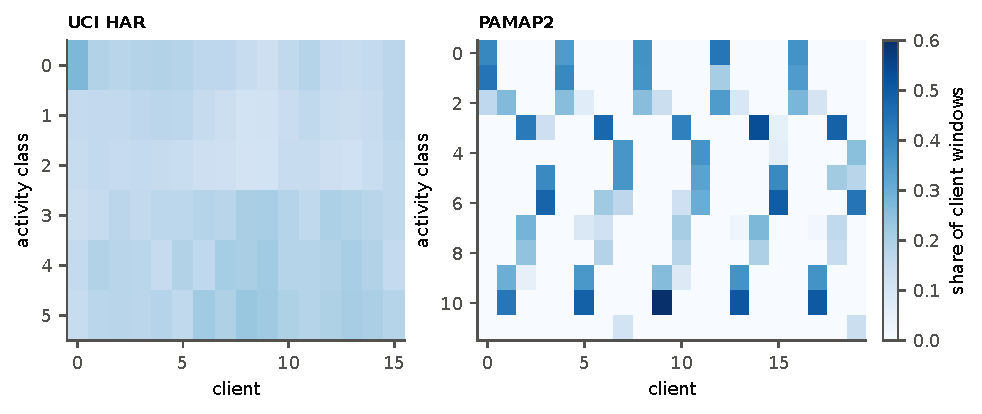
\includegraphics[width=0.95\textwidth]{fig_a1_noniid}
\caption{Share of each activity class in each client's training windows. UCI HAR clients are persons who all performed all activities; PAMAP2 clients are time chunks of a sequential protocol and hold three to five classes.}\label{fig:pamap-noniid}
\end{figure}

\subsection{Paired comparisons}\label{app:paired}
Tables~\ref{tab:p-ckpt}--\ref{tab:p-eta} give EcoFed minus baseline (or baseline/EcoFed for ratios), paired by seed, with bootstrap 95\% CIs and Holm-corrected $p$-values within each setting across the seven baselines; $^*$ marks $p<0.05$.
\begin{table}[h]\centering\scriptsize\caption{Best-checkpoint accuracy, EcoFed minus baseline (pp).}\label{tab:p-ckpt}\resizebox{\textwidth}{!}{\begin{tabular}{@{}llrrrr@{}}
\toprule
Data / $\phi$ & vs. & mean $\Delta$ (pp) & 95\% CI & $n$ & Holm $p$\\
\midrule
UCI HAR, 0.1 & Oort-style & -1.89 & [-3.91, 0.32] & 16 & 0.705\\
 & Energy-greedy & -2.20 & [-4.06, -0.23] & 16 & 0.344\\
 & Static-Depth & -0.28 & [-1.75, 1.20] & 16 & 0.987\\
 & FedAvg-Paced & -0.87 & [-2.76, 1.26] & 16 & 0.987\\
 & FedAvg-Q8 & -1.65 & [-3.89, 0.74] & 16 & 0.987\\
 & FedProx & -1.12 & [-2.98, 0.69] & 16 & 0.987\\
 & FedAvg & -1.36 & [-3.32, 0.77] & 16 & 0.987\\
\midrule
UCI HAR, 0.25 & Oort-style & -1.62 & [-3.03, -0.31] & 16 & 0.082\\
 & Energy-greedy & -2.12 & [-3.86, -0.54] & 16 & 0.080\\
 & Static-Depth & -1.10 & [-2.60, 0.40] & 16 & 0.183\\
 & FedAvg-Paced & -2.28$^{*}$ & [-3.76, -0.89] & 16 & 0.039\\
 & FedAvg-Q8 & -1.91 & [-3.32, -0.53] & 16 & 0.080\\
 & FedProx & -2.66$^{*}$ & [-3.96, -1.34] & 16 & 0.010\\
 & FedAvg & -2.36$^{*}$ & [-3.54, -1.19] & 16 & 0.010\\
\midrule
UCI HAR, 1.0 & Oort-style & -1.13 & [-2.09, -0.11] & 16 & 0.225\\
 & Energy-greedy & -1.30 & [-2.24, -0.30] & 16 & 0.129\\
 & Static-Depth & -0.07 & [-1.25, 1.23] & 16 & 1.000\\
 & FedAvg-Paced & -1.62 & [-2.73, -0.58] & 16 & 0.088\\
 & FedAvg-Q8 & -0.82 & [-1.89, 0.37] & 16 & 0.560\\
 & FedProx & -0.27 & [-1.48, 1.01] & 16 & 1.000\\
 & FedAvg & -1.11 & [-2.13, 0.00] & 16 & 0.260\\
\midrule
PAMAP2, 0.1 & Oort-style & 4.17 & [0.55, 7.85] & 16 & 0.114\\
 & Energy-greedy & 0.74 & [-3.41, 5.40] & 16 & 0.756\\
 & Static-Depth & -7.76 & [-12.82, -2.97] & 16 & 0.068\\
 & FedAvg-Paced & 5.99 & [1.64, 10.67] & 16 & 0.114\\
 & FedAvg-Q8 & 6.18 & [1.59, 10.75] & 16 & 0.114\\
 & FedProx & 5.17 & [1.25, 9.10] & 16 & 0.114\\
 & FedAvg & 6.51 & [2.37, 10.59] & 16 & 0.068\\
\midrule
PAMAP2, 0.25 & Oort-style & 10.91$^{*}$ & [6.33, 15.67] & 16 & 0.002\\
 & Energy-greedy & 7.31$^{*}$ & [3.81, 10.93] & 16 & 0.004\\
 & Static-Depth & 2.04 & [-2.25, 6.63] & 16 & 0.384\\
 & FedAvg-Paced & 7.92$^{*}$ & [4.22, 11.70] & 16 & 0.004\\
 & FedAvg-Q8 & 8.95$^{*}$ & [6.01, 11.60] & 16 & 0.000\\
 & FedProx & 8.76$^{*}$ & [5.56, 11.78] & 16 & 0.000\\
 & FedAvg & 9.99$^{*}$ & [6.96, 13.19] & 16 & 0.000\\
\midrule
PAMAP2, 1.0 & Oort-style & 3.97 & [0.23, 8.45] & 16 & 0.564\\
 & Energy-greedy & 3.18 & [0.05, 6.58] & 16 & 0.564\\
 & Static-Depth & -0.86 & [-4.97, 3.54] & 16 & 1.000\\
 & FedAvg-Paced & -0.28 & [-3.81, 3.11] & 16 & 1.000\\
 & FedAvg-Q8 & 5.15 & [0.21, 10.90] & 16 & 0.564\\
 & FedProx & 3.07 & [-1.68, 8.26] & 16 & 0.796\\
 & FedAvg & 4.06 & [-0.12, 8.56] & 16 & 0.564\\
\bottomrule
\end{tabular}}\end{table}
\begin{table}[h]\centering\scriptsize\caption{Final accuracy, EcoFed minus baseline (pp).}\label{tab:p-final}\resizebox{\textwidth}{!}{\begin{tabular}{@{}llrrrr@{}}
\toprule
Data / $\phi$ & vs. & mean $\Delta$ (pp) & 95\% CI & $n$ & Holm $p$\\
\midrule
UCI HAR, 0.1 & Oort-style & 1.85 & [-0.99, 5.12] & 16 & 0.912\\
 & Energy-greedy & 1.96 & [-0.45, 4.90] & 16 & 0.912\\
 & Static-Depth & 3.33 & [1.15, 5.83] & 16 & 0.114\\
 & FedAvg-Paced & 0.71 & [-1.59, 3.18] & 16 & 0.985\\
 & FedAvg-Q8 & 2.68 & [0.06, 5.87] & 16 & 0.625\\
 & FedProx & 0.89 & [-1.41, 3.38] & 16 & 0.985\\
 & FedAvg & 1.49 & [-0.59, 3.66] & 16 & 0.912\\
\midrule
UCI HAR, 0.25 & Oort-style & 1.90 & [-0.17, 3.98] & 16 & 0.462\\
 & Energy-greedy & 1.58 & [0.08, 3.10] & 16 & 0.425\\
 & Static-Depth & -0.17 & [-1.36, 1.11] & 16 & 0.800\\
 & FedAvg-Paced & -1.30 & [-2.59, 0.06] & 16 & 0.425\\
 & FedAvg-Q8 & 0.93 & [-0.36, 2.18] & 16 & 0.486\\
 & FedProx & 1.87 & [0.10, 3.64] & 16 & 0.425\\
 & FedAvg & 1.37 & [-0.34, 3.13] & 16 & 0.486\\
\midrule
UCI HAR, 1.0 & Oort-style & -0.53 & [-1.50, 0.46] & 16 & 1.000\\
 & Energy-greedy & -1.05 & [-2.04, -0.05] & 16 & 0.371\\
 & Static-Depth & -0.88 & [-1.79, 0.02] & 16 & 0.431\\
 & FedAvg-Paced & -1.81$^{*}$ & [-2.61, -1.07] & 16 & 0.004\\
 & FedAvg-Q8 & -0.12 & [-1.04, 0.79] & 16 & 1.000\\
 & FedProx & 0.30 & [-0.68, 1.24] & 16 & 1.000\\
 & FedAvg & -0.25 & [-1.27, 0.70] & 16 & 1.000\\
\midrule
PAMAP2, 0.1 & Oort-style & 11.80$^{*}$ & [7.00, 16.32] & 16 & 0.001\\
 & Energy-greedy & 13.53$^{*}$ & [9.25, 17.80] & 16 & 0.000\\
 & Static-Depth & 7.00$^{*}$ & [3.17, 11.26] & 16 & 0.006\\
 & FedAvg-Paced & 5.91$^{*}$ & [3.10, 8.96] & 16 & 0.003\\
 & FedAvg-Q8 & 12.98$^{*}$ & [9.33, 16.20] & 16 & 0.000\\
 & FedProx & 15.25$^{*}$ & [11.05, 19.49] & 16 & 0.000\\
 & FedAvg & 14.39$^{*}$ & [10.30, 18.23] & 16 & 0.000\\
\midrule
PAMAP2, 0.25 & Oort-style & 22.52$^{*}$ & [17.33, 28.14] & 16 & 0.000\\
 & Energy-greedy & 27.20$^{*}$ & [23.20, 31.50] & 16 & 0.000\\
 & Static-Depth & 12.08$^{*}$ & [8.32, 15.89] & 16 & 0.000\\
 & FedAvg-Paced & 10.39$^{*}$ & [5.71, 15.78] & 16 & 0.001\\
 & FedAvg-Q8 & 22.94$^{*}$ & [19.41, 26.70] & 16 & 0.000\\
 & FedProx & 23.02$^{*}$ & [18.89, 26.81] & 16 & 0.000\\
 & FedAvg & 20.69$^{*}$ & [16.78, 24.39] & 16 & 0.000\\
\midrule
PAMAP2, 1.0 & Oort-style & 8.51$^{*}$ & [4.47, 13.02] & 16 & 0.007\\
 & Energy-greedy & 5.67$^{*}$ & [2.01, 9.28] & 16 & 0.025\\
 & Static-Depth & -2.29 & [-5.31, 0.79] & 16 & 0.340\\
 & FedAvg-Paced & 0.89 & [-2.64, 4.56] & 16 & 0.649\\
 & FedAvg-Q8 & 11.93$^{*}$ & [6.90, 16.81] & 16 & 0.002\\
 & FedProx & 11.90$^{*}$ & [7.05, 16.26] & 16 & 0.001\\
 & FedAvg & 10.73$^{*}$ & [6.24, 14.88] & 16 & 0.001\\
\bottomrule
\end{tabular}}\end{table}
\begin{table}[h]\centering\scriptsize\caption{Total fleet energy used, ratio baseline/EcoFed.}\label{tab:p-energy}\resizebox{\textwidth}{!}{\begin{tabular}{@{}llrrrr@{}}
\toprule
Data / $\phi$ & vs. & mean ratio (baseline/EcoFed) & 95\% CI & $n$ & Holm $p$\\
\midrule
UCI HAR, 0.1 & Oort-style & 0.84$^{*}$ & [0.83, 0.84] & 16 & 0.000\\
 & Energy-greedy & 0.84$^{*}$ & [0.83, 0.84] & 16 & 0.000\\
 & Static-Depth & 1.12$^{*}$ & [1.11, 1.13] & 16 & 0.000\\
 & FedAvg-Paced & 0.84$^{*}$ & [0.83, 0.84] & 16 & 0.000\\
 & FedAvg-Q8 & 0.85$^{*}$ & [0.85, 0.86] & 16 & 0.000\\
 & FedProx & 0.84$^{*}$ & [0.83, 0.84] & 16 & 0.000\\
 & FedAvg & 0.84$^{*}$ & [0.83, 0.84] & 16 & 0.000\\
\midrule
UCI HAR, 0.25 & Oort-style & 1.64$^{*}$ & [1.61, 1.68] & 16 & 0.000\\
 & Energy-greedy & 1.64$^{*}$ & [1.61, 1.68] & 16 & 0.000\\
 & Static-Depth & 1.52$^{*}$ & [1.49, 1.56] & 16 & 0.000\\
 & FedAvg-Paced & 1.64$^{*}$ & [1.61, 1.68] & 16 & 0.000\\
 & FedAvg-Q8 & 1.69$^{*}$ & [1.67, 1.72] & 16 & 0.000\\
 & FedProx & 1.64$^{*}$ & [1.61, 1.68] & 16 & 0.000\\
 & FedAvg & 1.64$^{*}$ & [1.61, 1.68] & 16 & 0.000\\
\midrule
UCI HAR, 1.0 & Oort-style & 2.14$^{*}$ & [2.07, 2.19] & 16 & 0.000\\
 & Energy-greedy & 1.96$^{*}$ & [1.92, 2.00] & 16 & 0.000\\
 & Static-Depth & 1.53$^{*}$ & [1.50, 1.55] & 16 & 0.000\\
 & FedAvg-Paced & 2.21$^{*}$ & [2.18, 2.23] & 16 & 0.000\\
 & FedAvg-Q8 & 2.00$^{*}$ & [1.98, 2.03] & 16 & 0.000\\
 & FedProx & 2.15$^{*}$ & [2.12, 2.18] & 16 & 0.000\\
 & FedAvg & 2.15$^{*}$ & [2.12, 2.18] & 16 & 0.000\\
\midrule
PAMAP2, 0.1 & Oort-style & 1.42$^{*}$ & [1.35, 1.49] & 16 & 0.000\\
 & Energy-greedy & 1.42$^{*}$ & [1.35, 1.49] & 16 & 0.000\\
 & Static-Depth & 1.94$^{*}$ & [1.90, 1.99] & 16 & 0.000\\
 & FedAvg-Paced & 1.42$^{*}$ & [1.35, 1.49] & 16 & 0.000\\
 & FedAvg-Q8 & 1.45$^{*}$ & [1.39, 1.53] & 16 & 0.000\\
 & FedProx & 1.42$^{*}$ & [1.35, 1.49] & 16 & 0.000\\
 & FedAvg & 1.42$^{*}$ & [1.35, 1.49] & 16 & 0.000\\
\midrule
PAMAP2, 0.25 & Oort-style & 0.92$^{*}$ & [0.91, 0.93] & 16 & 0.000\\
 & Energy-greedy & 0.92$^{*}$ & [0.91, 0.93] & 16 & 0.000\\
 & Static-Depth & 1.16$^{*}$ & [1.15, 1.17] & 16 & 0.000\\
 & FedAvg-Paced & 0.92$^{*}$ & [0.91, 0.93] & 16 & 0.000\\
 & FedAvg-Q8 & 0.92$^{*}$ & [0.91, 0.93] & 16 & 0.000\\
 & FedProx & 0.92$^{*}$ & [0.91, 0.93] & 16 & 0.000\\
 & FedAvg & 0.92$^{*}$ & [0.91, 0.93] & 16 & 0.000\\
\midrule
PAMAP2, 1.0 & Oort-style & 1.20$^{*}$ & [1.18, 1.22] & 16 & 0.000\\
 & Energy-greedy & 1.08$^{*}$ & [1.06, 1.10] & 16 & 0.000\\
 & Static-Depth & 0.99 & [0.97, 1.01] & 16 & 0.528\\
 & FedAvg-Paced & 1.21$^{*}$ & [1.19, 1.22] & 16 & 0.000\\
 & FedAvg-Q8 & 1.11$^{*}$ & [1.10, 1.12] & 16 & 0.000\\
 & FedProx & 1.18$^{*}$ & [1.16, 1.19] & 16 & 0.000\\
 & FedAvg & 1.18$^{*}$ & [1.16, 1.19] & 16 & 0.000\\
\bottomrule
\end{tabular}}\end{table}
\begin{table}[h]\centering\scriptsize\caption{Energy to reach 90\% of the plateau, ratio baseline/EcoFed (seeds that reach it in both).}\label{tab:p-eta}\resizebox{\textwidth}{!}{\begin{tabular}{@{}llrrrr@{}}
\toprule
Data / $\phi$ & vs. & mean ratio (baseline/EcoFed) & 95\% CI & $n$ & Holm $p$\\
\midrule
UCI HAR, 0.1 & Oort-style & 2.17$^{*}$ & [1.86, 2.45] & 16 & 0.000\\
 & Energy-greedy & 1.63$^{*}$ & [1.33, 1.93] & 16 & 0.023\\
 & Static-Depth & 1.02 & [0.74, 1.34] & 16 & 0.331\\
 & FedAvg-Paced & 1.43 & [1.17, 1.68] & 16 & 0.064\\
 & FedAvg-Q8 & 1.85$^{*}$ & [1.49, 2.20] & 16 & 0.006\\
 & FedProx & 2.14$^{*}$ & [1.78, 2.49] & 16 & 0.000\\
 & FedAvg & 1.74$^{*}$ & [1.42, 2.07] & 16 & 0.006\\
\midrule
UCI HAR, 0.25 & Oort-style & 1.79$^{*}$ & [1.39, 2.20] & 16 & 0.026\\
 & Energy-greedy & 1.77$^{*}$ & [1.37, 2.19] & 16 & 0.011\\
 & Static-Depth & 1.21 & [0.97, 1.46] & 16 & 0.508\\
 & FedAvg-Paced & 3.70$^{*}$ & [3.03, 4.42] & 16 & 0.000\\
 & FedAvg-Q8 & 3.19$^{*}$ & [2.68, 3.69] & 16 & 0.000\\
 & FedProx & 3.77$^{*}$ & [2.99, 4.57] & 16 & 0.000\\
 & FedAvg & 3.34$^{*}$ & [2.62, 4.12] & 16 & 0.000\\
\midrule
UCI HAR, 1.0 & Oort-style & 0.80 & [0.64, 0.96] & 16 & 0.063\\
 & Energy-greedy & 0.82 & [0.65, 1.03] & 16 & 0.063\\
 & Static-Depth & 1.19 & [0.98, 1.46] & 16 & 0.273\\
 & FedAvg-Paced & 1.80$^{*}$ & [1.58, 2.01] & 16 & 0.000\\
 & FedAvg-Q8 & 1.69$^{*}$ & [1.42, 1.96] & 16 & 0.000\\
 & FedProx & 1.72$^{*}$ & [1.43, 1.99] & 16 & 0.004\\
 & FedAvg & 1.72$^{*}$ & [1.42, 2.01] & 16 & 0.004\\
\midrule
PAMAP2, 0.1 & Oort-style & 4.15 & [1.97, 7.14] & 3 & 0.300\\
 & Energy-greedy & 3.50$^{*}$ & [2.31, 4.96] & 6 & 0.017\\
 & Static-Depth & 1.58 & [1.00, 2.28] & 9 & 0.300\\
 & FedAvg-Paced & 4.60$^{*}$ & [2.70, 7.13] & 5 & 0.036\\
 & FedAvg-Q8 & 4.20 & [1.78, 7.19] & 3 & 0.300\\
 & FedProx & 4.30 & [1.95, 7.88] & 3 & 0.300\\
 & FedAvg & 3.87 & [2.19, 6.46] & 4 & 0.141\\
\midrule
PAMAP2, 0.25 & Oort-style & 2.33$^{*}$ & [1.70, 3.05] & 14 & 0.002\\
 & Energy-greedy & 1.92$^{*}$ & [1.57, 2.29] & 14 & 0.000\\
 & Static-Depth & 1.02 & [0.70, 1.37] & 15 & 0.283\\
 & FedAvg-Paced & 2.17$^{*}$ & [1.34, 3.26] & 13 & 0.043\\
 & FedAvg-Q8 & 2.14$^{*}$ & [1.61, 2.75] & 15 & 0.003\\
 & FedProx & 2.51$^{*}$ & [1.92, 3.15] & 14 & 0.000\\
 & FedAvg & 2.52$^{*}$ & [1.86, 3.24] & 15 & 0.000\\
\midrule
PAMAP2, 1.0 & Oort-style & 1.42$^{*}$ & [1.18, 1.73] & 15 & 0.016\\
 & Energy-greedy & 1.21 & [0.93, 1.53] & 15 & 1.000\\
 & Static-Depth & 1.15 & [0.87, 1.49] & 15 & 1.000\\
 & FedAvg-Paced & 1.76$^{*}$ & [1.31, 2.33] & 15 & 0.010\\
 & FedAvg-Q8 & 1.90$^{*}$ & [1.63, 2.20] & 15 & 0.000\\
 & FedProx & 1.98$^{*}$ & [1.67, 2.30] & 15 & 0.000\\
 & FedAvg & 1.97$^{*}$ & [1.66, 2.31] & 15 & 0.000\\
\bottomrule
\end{tabular}}\end{table}

\subsection{Accuracy per exit}
\begin{table}[h]\centering\scriptsize\caption{Test accuracy (\%) of each exit at the end of training, $\phi=0.25$, mean over 16 seeds. Single-exit FedAvg trains only the last exit.}\label{tab:exits}\resizebox{0.8\textwidth}{!}{\begin{tabular}{@{}llrrrr@{}}
\toprule
Data / $\phi$ & Method & Exit 1 & Exit 2 & Exit 3 & Exit 4\\
\midrule
UCI HAR, 0.25 & EcoFed & 85.3 & 84.4 & 84.9 & 85.0\\
 & Static-Depth & 85.8 & 85.3 & 85.8 & 81.2\\
 & Oort-style & 57.5 & 82.1 & 83.8 & 84.2\\
 & FedAvg & 55.9 & 82.9 & 84.3 & 84.7\\
 & FedAvg (single exit) & 15.1 & 15.2 & 15.2 & 87.2\\
\midrule
PAMAP2, 0.25 & EcoFed & 57.5 & 52.3 & 46.9 & 44.4\\
 & Static-Depth & 44.5 & 32.8 & 30.2 & 28.1\\
 & Oort-style & 27.5 & 31.6 & 29.1 & 27.7\\
 & FedAvg & 24.5 & 35.5 & 29.9 & 28.8\\
 & FedAvg (single exit) & 8.2 & 6.5 & 8.0 & 31.4\\
\bottomrule
\end{tabular}}\end{table}

\subsection{Pilot on exit weighting}
In a pilot on tuning seeds (UCI HAR, FedAvg, 4 seeds) uniform exit weights gave a validation accuracy at the end of the budget of 81.9\% at $\phi=0.1$ and 87.5\% at $\phi=1$, whereas weights proportional to $j^2$ gave 85.1\% and 88.5\%, and a single-exit objective gave 86.4\% and 88.6\%; the single-exit model was clearly worse early in the run (68.9\% against 79.6\% at 25\% of the capacity for the uniform weighting at $\phi=0.1$). We therefore use $\lambda_j\propto j^2$ for all methods. Hyper-parameters were tuned after this decision.

\subsection{Code and data}
Everything needed to regenerate the tables and figures is in the repository: loaders for both datasets, the model, the energy model, the simulator, all methods, experiment configurations, tuned hyper-parameters and the analysis scripts. Raw per-run logs are regenerated by the experiment scripts (they are not committed because of their size).

\end{document}
